% start the document

% specify the document layout and font size
\documentclass[preprint,12pt]{elsarticle}
% \documentclass[final,twocolumn,12pt]{elsarticle}
% \usepackage[margin=1.5cm,includefoot]{geometry}
\usepackage{setspace}

% uploading packages
\usepackage{graphicx}
\usepackage{amssymb}
\usepackage{textcomp} % https://latex.org/forum/viewtopic.php?f=4&t=3364#p13124, https://tex.stackexchange.com/questions/165115
\usepackage{gensymb}
\usepackage{lineno}
\usepackage{mathtools}
\usepackage[title]{appendix}
\usepackage{pgfmath}
\newcommand{\calcnum}[1]{%
    \pgfmathparse{#1}%
    \num[round-mode=places,round-precision=1]{\pgfmathresult}%
}
\usepackage[separate-uncertainty=true]{siunitx} % \usepackage{xr-hyper} %needs to  be before hyperref
\usepackage{xurl} %needs to be before hyperref
\usepackage[colorlinks]{hyperref}
\hypersetup{breaklinks=true} % set automatically by hyperref?
% \PassOptionsToPackage{hyphens}{url}\usepackage{hyperref} %allow URLs to break across lines
\usepackage[nameinlink,capitalise]{cleveref} %needs to appear after hyperref, https://tex.stackexchange.com/questions/396728/my-equations-referencing-not-working
\Crefname{figure}{Figure}{Figures} %needs to appear after hyperref and cleveref
\crefname{appsec}{Appendix}{Appendices}
\newcommand\crefrangeconjunction{--} % modify the reference style
\usepackage{mathrsfs}
\usepackage{enumitem}
\usepackage{tabulary}
\usepackage{caption}
\usepackage{subcaption}
\usepackage{multirow}
\usepackage{makecell} % https://tex.stackexchange.com/questions/2441/how-to-add-a-forced-line-break-inside-a-table-cell
\newcommand{\NA}{---} % holds an m-dash
\graphicspath{{figures/}} %Setting the graphicspath
% ---------to deal with the double quotes----------- 
\usepackage [english]{babel}
\usepackage [autostyle, english = american]{csquotes}
\MakeOuterQuote{"}
\usepackage{listings}[breakatwhitespace=true,escapechar=\%]
\usepackage{matlab-prettifier}
\newcommand{\matlab}[1]{\mbox{\lstinline[style=Matlab-editor]{#1}}}
%alternatively can use `` '' format for double quotes
\usepackage{booktabs}
\setlength{\abovetopsep}{1ex}
\usepackage[shortcuts,abbreviations]{glossaries-extra}
\newcommand*{\TCac}[1]{\ecapitalisewords{\glsentrylong{#1}}}
% remove the "Preprint submitted to Elsevier" footer on the first page
\makeatletter
\def\ps@pprintTitle{%
   \let\@oddhead\@empty
   \let\@evenhead\@empty
   \def\@oddfoot{\reset@font\hfil\thepage\hfil}
   \let\@evenfoot\@oddfoot
}
\makeatother

% Cross referencing with the xr package in Overleaf (https://www.overleaf.com/learn/how-to/Cross_referencing_with_the_xr_package_in_Overleaf)
\makeatletter
\newcommand*{\addFileDependency}[1]{% argument=file name and extension
  \typeout{(#1)}
  \@addtofilelist{#1}
  \IfFileExists{#1}{}{\typeout{No file #1.}}
}
\makeatother
\newcommand*{\myexternaldocument}[1]{%
    \externaldocument{#1}%
    \addFileDependency{#1.tex}%
    \addFileDependency{#1.aux}%
}

\usepackage{nameref,zref-xr}
\zxrsetup{toltxlabel}
%https://tex.stackexchange.com/questions/77774/undefined-control-sequence-when-cross-referencing-with-xr-hyper
% \myexternaldocument{supp}

\biboptions{sort&compress}
\interfootnotelinepenalty=10000 %prevent footnotes from getting split across columns/pages 
%\patchcmd{\emailauthor}{(#2)}{(S.G. Baird).}{}{} %Removes/Abbreviates corresponding author name after Email address so that the footnote doesn't take up 2 lines.
% Double Spacing
% \doublespacing
\usepackage[margin=1.5cm,includefoot]{geometry}
\usepackage{auto-paper}
% \PassOptionsToPackage{refcheck}{auto-paper} %comment this out before submission

\zexternaldocument*{main-frankenstein-2} %try deleting log files if producing an error, see https://tex.stackexchange.com/questions/131709/unclean-aux-file-causes-file-ended-while-scanning-use-of-newlbel-error-wh
% Concatenate the different "values" .tex files
%RMSE values
% \newcommand{\baryrmse}{0.0242}
% \newcommand{\gprrmse}{0.0220}
% \newcommand{\idwrmse}{0.0345}
% \newcommand{\nnrmse}{0.0448}
% \newcommand{\avgrmse}{0.1302}
% %paper-data6
% \newcommand{\baryrmse}{0.0238}
% \newcommand{\gprrmse}{0.0218}
% \newcommand{\idwrmse}{0.0356}
% \newcommand{\nnrmse}{0.0445}
% \newcommand{\avgrmse}{0.1283}
%\newcommand{\gprrmsePercReduction}{83}
% paper-data9
\newcommand{\baryrmse}{0.0239}
\newcommand{\gprrmse}{0.0217}
\newcommand{\idwrmse}{0.0343}
\newcommand{\nnrmse}{0.0448}
\newcommand{\avgrmse}{0.1284}
\newcommand{\gprrmsePercReduction}{83.1}

%MAE values
% \newcommand{\barymae}{0.0145}
% \newcommand{\gprmae}{0.0145}
% \newcommand{\idwmae}{0.0223}
% \newcommand{\nnmae}{0.0307}
% \newcommand{\avgmae}{0.0965}
% %paper-data6
% \newcommand{\barymae}{0.0145}
% \newcommand{\gprmae}{0.0145}
% \newcommand{\idwmae}{0.0225}
% \newcommand{\nnmae}{0.0307}
% \newcommand{\avgmae}{0.0955}
%paper-data9
\newcommand{\barymae}{0.0145}
\newcommand{\gprmae}{0.0145}
\newcommand{\idwmae}{0.0223}
\newcommand{\nnmae}{0.0308}
\newcommand{\avgmae}{0.0959}

%\newcommand{\nnomega}{2.8709 \pm 0.69112}
\newcommand{\nnomega}{2.8702 \pm 0.69117}

\newcommand{\symtime}{76}

\newcommand{\nigprbrkrmse}{0.1471}

%Supplementary
\newcommand{\thr}{\SI{1.1}{\joule\per\square\meter}}
\newcommand{\sigthr}{\SI{1.1}{\joule\per\square\meter}}
\newcommand{\thrtwo}{\SI{1.2}{\joule\per\square\meter}}


%% main-frankenstein-2
\newcommand{\minsymdist}{$\sim$\SI{64.0}{\tobydeg}}
\newcommand{\percExplained}{$\sim$\SI{99.6}{\percent}}
\newcommand{\percFiveVsOne}{$\sim$\SI{70}{\percent}}
\newcommand{\dimOne}{$\sim$\SI{65}{\tobydeg}}

% figure info, etc. that can dynamically change (color of points, etc.)
\newcommand{\startpt}{red points}
\newcommand{\singlept}{magenta points}
\newcommand{\sympt}{dark blue points}
\newcommand{\singlesympt}{dark blue point}
\newcommand{\refpt}{white circle}
\newcommand{\vbordercolor}{black}
\newcommand{\vcellcolor}{light blue}
\newcommand{\inpt}{input}
\newcommand{\outpt}{prediction}
% \newcommand{\inptvar}{ninputpts}
% \newcommand{\distfn}{GBdist4}
\newcommand{\vfzorepo}{\gls{vfz} repository}
\newcommand{\mytitleone}{Five Degree-of-Freedom Property Interpolation of Arbitrary Grain Boundaries via \glsentrytitlecase{vfz}{long} Framework}
% \newcommand{\mytitletwo}{Properties of a \glsentrytitlecase{5dof}{long} \glsentrytitlecase{fz}{long} defined via \glsentrytitlecase{vfz}{long} Framework}
\newcommand{\mytitletwo}{$O_h$ \glsentrytitlecase{5dof}{long} \glsentrytitlecase{fz}{long} Properties via \glsentrytitlecase{vfz}{long} Framework}
\makeglossaries
\GlsXtrEnableEntryCounting{abbreviation}{3}
% \glssetcategoryattribute{abbreviation}{indexonlyfirst}{true}
\glssetcategoryattribute{abbreviation}{nohyper}{true}

% \setabbreviationstyle[abbreviation]{long-short}

% \glsenableentrycount
% \glssetcategoryattribute{abbreviation}{entrycount}{2}

\newabbreviation[longplural=five degrees of freedom]{5dof}{5DOF}{five degree-of-freedom}
\newabbreviation[longplural=three degrees of freedom]{3dof}{3DOF}{three degree-of-freedom}
\newabbreviation[longplural=degrees of freedom]{dof}{DOF}{degree of freedom}
\newabbreviation{ebsd}{EBSD}{electron backscatter diffraction}
\newabbreviation[longplural={grain boundaries}]{gb}{GB}{grain boundary}
\newabbreviation{fcc}{FCC}{face-centered cubic}
\newabbreviation{sem}{SEM}{scanning electron microscope}
\newabbreviation{fea}{FEA}{finite element analysis}
\newabbreviation{bcs}{BCs}{boundary conditions}
\newabbreviation[longplural={triple junctions}]{tj}{TJ}{triple junction}
\newabbreviation{gpr}{GPR}{Gaussian process regression}
\newabbreviation{gprm}{GPRM}{Gaussian process regression mixture}
\newabbreviation{ann}{ANN}{artificial neural network}
\newabbreviation{nn}{NN}{nearest neighbor}
\newabbreviation{rmse}{RMSE}{root mean square error}
\newabbreviation{mae}{MAE}{mean absolute error}
\newabbreviation{brk}{BRK}{Bulatov Reed Kumar}
\newabbreviation{gbed}{GBED}{grain boundary energy distribution}
\newabbreviation{gbcd}{GBCD}{grain boundary character distribution}
\newabbreviation{mfz}{MFZ}{misorientation fundamental zone}
\newabbreviation{bp}{BP}{boundary plane}
\newabbreviation{bpfz}{BPFZ}{boundary plane fundamental zone}
\newabbreviation{knn}{kNN}{k-nearest neighbor}
\newabbreviation{gbe}{GBE}{grain boundary energy}
\newabbreviation{gbo}{GBO}{grain boundary octonion}
\newabbreviation{nbo}{NBO}{no-boundary octonion}
\newabbreviation{oslerp}{oSLERP}{octonion Spherical Linear Interpolation}
\newabbreviation{loocv}{LOOCV}{leave-one-out cross validation}
\newabbreviation{kfcv}{kFCV}{k-fold cross validation}
\newabbreviation{seo}{SEO}{symmetrically equivalent octonion}
\newabbreviation{fex}{FEX}{file exchange}
\newabbreviation{idw}{IDW}{inverse-distance weighting}
\newabbreviation{fic}{FIC}{fully independent conditional}
\newabbreviation{svd}{SVD}{singular value decomposition}
\newabbreviation{gbc}{GBC}{grain boundary character}
\newabbreviation{fz}{FZ}{fundamental zone}
% \newabbreviation{pfz}{pFZ}{pseudo fundamental zone} % pfz replaced by vfz
% \newabbreviation{cmo}{CMO}{closed-mesh octonion} % cmo replaced by vfzo
\newabbreviation{vfz}{VFZ}{Voronoi fundamental zone}
\newabbreviation{vfzgbo}{VFZ-GBO}{Voronoi fundamental zone grain boundary octonion}
\newabbreviation{lobpcg}{LOBPCG}{locally optimal block preconditioned conjugate gradient}
\newabbreviation{lkr}{LKR}{Laplacian kernel regression}
\newabbreviation{ms}{MS}{molecular statics}
\newabbreviation{sst}{SST}{standard stereographic triangle}
\newabbreviation{ml}{ML}{machine learning}
\newabbreviation{doe}{DoE}{design of experiments}
\newabbreviation{ct}{CT}{coherent-twin}
% example abbreviations
% \newabbreviation{seo}{SEO}{symmetrically equivalent octonions}
%\newabbreviation[longplural={grain boundaries}]{gb}{GB}{grain boundary}

%example usage: \gls{gpr}
%example usage: \Gls{gpr} (capitalize first letter, only meaningful for first usage)
% \glspl{seo} --> symmetrically equivalent octonions OR SEOs
%^^^^^^^^^^^^^^^^^^^^^^^^^^^^^^^^^^^^^^^^^^^^^^^^^^^


% Add "S" to figure captions, sections, and equations
\renewcommand{\thefigure}{S\arabic{figure}}
\renewcommand{\thesection}{S\arabic{section}}
\renewcommand{\theequation}{S\arabic{equation}}

\begin{document}
	\sloppy %maybe deals with figure/text spacing. Should deal with text going off the page
	
	\begin{frontmatter}
		
		%\title{Grain Boundary Octonion Meshing and Interpolation}
		\title{\mytitletwo{}: Supplementary Information}
		
		\author[myu]{Sterling G. Baird\corref{cor1}}
\ead{ster.g.baird@gmail.com}
\author[myu]{Eric R. Homer}
\author[myu]{David T. Fullwood}
\author[myu]{Oliver K. Johnson}

\address[myu]{Department of Mechanical Engineering, Brigham Young University, Provo, UT 84602, USA}

\cortext[cor1]{Corresponding author.}

\date{October 2021}
		
	\end{frontmatter}
	
\tableofcontents

\section{Brief Summary of \glsxtrshort{vfz} Methods}

We summarize the following aspects of the \gls{vfz} framework:
\begin{itemize}
    \item Creation and definition of a \gls{vfz}
    \item Mapping \glspl{gb} to the \gls{vfz}
    \item Distance calculations
    \item Interpolation
    \item Comparison with traditional \gls{gbo} metric
\end{itemize}
Each of these is described in greater detail in \citet{bairdFiveDegreeofFreedomPropertyUnderReview}.
%
% 	\subsection{Defining the \glsentrytitlecase{vfz}{long}} \label{sec:methods:framework:vfz}
	%
	%\Gls{3dof} \glspl{fz} have typically been defined using linear inequalities (e.g. the orientation \cite{heinzRepresentationOrientationDisorientation1991} and misorientation \cite{grimmerUniqueDescriptionRelative1980,heinzRepresentationOrientationDisorientation1991} \glspl{fz}). Instead of using linear inequalities\footnote{If desired, linear inequalities can be obtained for a \gls{vfz} by determining a Voronoi tessellation's junction points (similar to what is shown in \cref{fig:voronoi} by e.g. \matlab{voronoin()}), transforming to 6D Cartesian coordinates via a \gls{svd} transformation (\cref{sec:app:bary}) and defining the bounded region by e.g. MATLAB FEX function \matlab{vert2lcon.m}.}, we take a numerical approach to define what we will call a \gls{vfz}.
	%
	To define a \gls{vfz}, an arbitrary, fixed, low-symmetry reference \gls{gbo} is chosen ($o_{\text{ref}}$) and for our use of \glspl{gbo}, the \gls{vfz} is defined as the region of $\mathbb{S}^7$ (the unit 7-sphere in 8 dimensions) closer to $o_{\text{ref}}$ than any of its symmetric images. %\footnote{We also refer to lower-dimensional representations of the 8D Cartesian \gls{vfz} as \glspl{vfz} (described in \cref{sec:methods:framework:proj}) and describe which dimensionality we are referring to as appropriate. }. However, use of the \gls{vfz} does not require its explicit construction. Rather, practical calculations require only the selection of the single point $o_{\text{ref}}$ (which completes the definition of the \gls{vfz}), followed by mapping of query points into the \gls{vfz} by comparison of their \glspl{seo} with $o_{\text{ref}}$.
	If a low-symmetry \gls{gb} is chosen, the point within a \gls{vfz} will be unique within numerical tolerance (and hence it is a true \gls{fz}). Additionally, we use a Euclidean approximation to the true geodesic distance.
	%To illustrate the process of mapping points into the \gls{vfz}, we describe a 3D Cartesian analogue (\cref{fig:voronoi}) to a 7D Cartesian non-degenerate (i.e. U(1) degeneracy removed) representation of a \gls{vfz}, which produces the \gls{sst} \cite{patalaSymmetriesRepresentationGrain2013} for the $O_h$ point group. A set of \num{500} points ($p_i, i\in[1,500]$) randomly scattered on the surface of the 2-sphere comprise the data (\startpt{} in \cref{fig:voronoi}a). A random point, $p_{\text{ref}}$, also on the surface of the 2-sphere, is chosen as the reference point (\refpt{}). In this illustration, $O_h$ or $m\bar{3}m$ point group rotations are used as symmetry operators, $S_j,\ j\in[1,N_p]$, where $N_p$ is the twice the number of proper rotations due to inversion symmetry and $N_p = 48$ for the $O_h$  point group. For each data point, \num{48} symmetrically equivalent representations ($p^{\text{sym}}_{i,j} = S_j(p_i),\ j\in[1,24]$) are produced by applying each of the relevant symmetry operators. After calculating the Euclidean distance between $p_{\text{ref}}$ and $p^{\text{sym}}_{i,j}$, the point ($p^{*}_i$) closest to $p_{\text{ref}}$ is chosen and retained as the unique representative of $p^{\text{sym}}_{i,j}$. As illustrated in \cref{fig:voronoi}a, the projected points $p^{*}_i$ (dark blue points) all fall in the \gls{vfz} without ever having to construct or define it explicitly. We call this group of projected points a \textit{\gls{vfz} point set}. Note also that there is only one $p^{*}_i$ in the \gls{vfz} for each $p^{\text{sym}}_{i,j}$ (see \cref{fig:voronoi}b).
	
%	\begin{figure*}
%		\centering
%		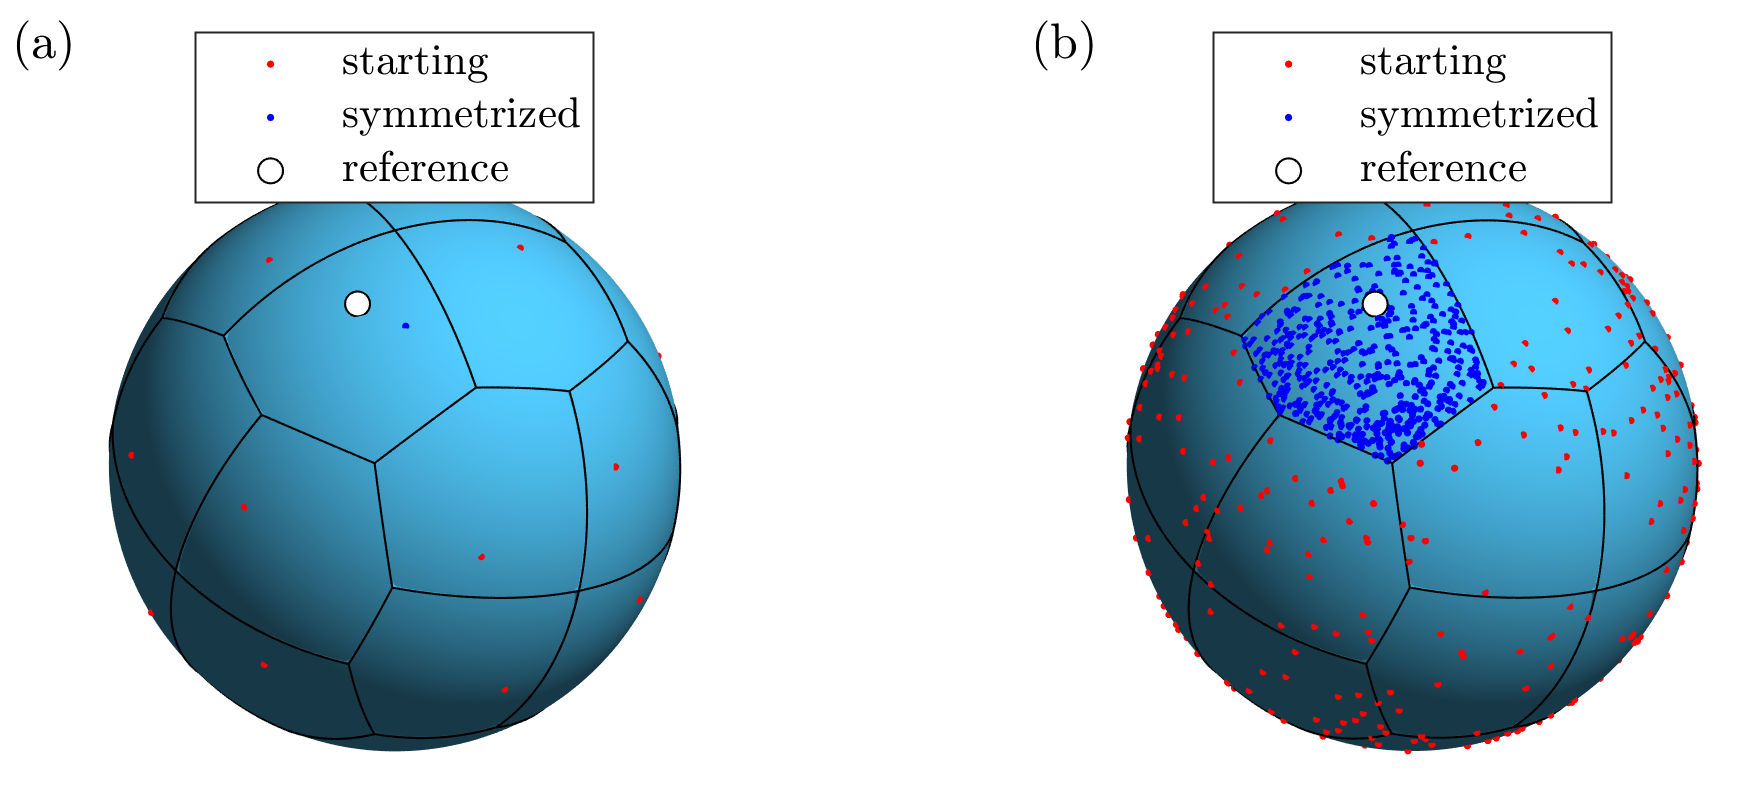
\includegraphics[scale=1]{voronoi.png}
%		\caption{(a) 3D Cartesian analogue to a non-degenerate 7D Cartesian representation of U(1)-symmetrized \glspl{gbo} and \glspl{vfzgbo} (\glspl{vfzgbo} are inherently U(1)-symmetrized) which demonstrates the symmetrization of many points relative to a fixed reference point (\refpt{}). This produces a 3D Cartesian \gls{vfz} point set (\sympt{}). (b) To further illustrate, a single input point (\singlept{}) is symmetrized (\singlesympt{}) relative to a fixed reference point (\refpt{}), demonstrating that only one symmetrized point is found within the borders (\vbordercolor{}) of each of the Voronoi cells (\vcellcolor{}). The Voronoi tessellation is defined by the symmetric images of the reference point, and the spherical Voronoi diagram for this illustration is constructed using a modified version of \cite{luongVoronoiSphere2020}.}
%		\label{fig:voronoi}
%	\end{figure*}
%
%	To calculate the distance between a given \gls{gbo}, and the reference \gls{gbo}, we employ the standard 8D Euclidean distance
%	\begin{equation}
%		\label{eq:8Deuclidean_dist}
%		d_{\text{E}}\!\left(o_{A},o_{B}\right) = {\left(\sum_{k=1}^{8} {\left(o_{A,k} - o_{B,k}\right)}^2 \right)}^{1/2}
%		%why not just
%		%\lVert o_A-o_B \rVert
%	\end{equation}
%	where $o_{A,k}$ and $o_{B,k}$ represent the $k$-the element of normalized \glspl{gbo} $o_A$, and $o_B$, respectively. 
%
%	Euclidean distance is an approximation to the true geodesic arc length on $\mathbb{S}^7$, which is given by
%	\begin{equation}
%		\label{eq:7sphere_arc_length}
%		d_{\text{S}}\!\left(o_{A},o_{B}\right)=\cos ^{-1}\left(o_A\cdot o_B\right)
%	\end{equation}
%	where $\cdot$ is the dot product, $\cos ^{-1}$ is the inverse cosine operator, and $o_A$ and $o_B$ are each normalized and $d_{\text{S}}\simeq d_{\text{E}}$ (\cref{fig:dist-parity}). In \cite{francisGeodesicOctonionMetric2019}, the original \gls{gbo} distance metric was defined by
%	\begin{equation}
%		\label{eq:omega}
%		d_\Omega\!\left(o_{A},o_{B}\right) = 2\cos ^{-1}\left(o_A\cdot o_B\right)
%	\end{equation}
%	where $o_A$ and $o_B$ are each normalized and $d_\Omega$ can be seen to be simply twice the geodesic arc length: $d_\Omega = 2 d_{\text{S}}$. Thus,
%	$d_\text{E}\simeq \frac{1}{2}d_\Omega$.
%	
%	The definition of $d_\Omega$ has certain aesthetic benefits in that it mirrors the definition of a misorientation angle, $\omega_{AB}$, between two crystal orientations in the quaternion parameterization: $\omega_{AB} = 2 \cos^{-1}{\left(q_A \cdot q_B\right)}$.
%	
%	Our choice to use $d_{\text{E}}$ instead of $d_{\text{S}}$ or $d_\Omega$ is motivated by the fact that it enables the use of standard algorithms, for a variety of operations, that require or assume Euclidean distances. In addition to enabling us to leverage the machinery of efficient and established algorithms, this choice can be justified by the following observations:
%	\begin{itemize}
%		\item The minimum Euclidean distance \gls{seo} will be the same as the minimum arc length distance \gls{seo} because $d_{\text{S}}$ is a monotonically increasing function of $d_{\text{E}}$, for $d_{\text{S}}\!\left(d_{\text{E}}\right)\in[0,\pi]$ (\cref{fig:dist-parity}). 
%		\item For the FCC point group symmetry ($m\bar{3}m$) the portion of $\mathbb{S}^7$ subtended by the \gls{vfz} is sufficiently small that the approximation $d_{\text{E}} \simeq d_{\text{S}}$ holds to very high accuracy\footnote{This is true for a specific pair of \glspl{gbo} within a \gls{vfz}. When calculating the \emph{minimum} distance between \glspl{seo} of two points, there are additional considerations that must be attended to as discussed in detail in \cref{sec:methods:framework:vfz-dist}.} as shown in \cref{fig:dist-parity}. 
%		\item Calculation of $d_{\text{E}}$ does not require the use of any inverse trigonometric functions and is about \SI{23}{\percent} faster than calculation of $d_{\text{S}}$ or $d_\Omega$.
%	\end{itemize}
%	
	%For applications other than interpolation which require precise quantification of high-dimensional volume, a mapping between Euclidean-approximated volumes and true volumes may be necessary\footnote{We have not tested to what extent a Euclidean-approximated volume will differ from the true volume; however, Euclidean-approximated volumes can be obtained by using the triangulation methods discussed in \cref{sec:app:bary:tri} (i.e. \matlab{convhulln()}).} or the Euclidean approximation may be removed altogether\footnote{i.e. by setting the \matlab{dtype} argument of \matlab{GBdist4.m} to \matlab{'omega'} rather than \matlab{'norm'}.}. The latter combined with removal of the renormalization of \gls{gbo} allows for the (non-ensembled) \gls{vfzgbo} metric to be intrinsic (see \citet{morawiecDistancesGrainInterfaces2019} for an in-depth treatment of intrinsicality).
%	
	%The expectation that a single, unique \gls{seo} will be found (within numerical tolerance and given a low-symmetry reference \gls{gbo}\footnote{The probability that a randomly generated \gls{gbo} will fall exactly on a high-symmetry boundary vanishes in the limit of infinite precision. }) is verified by several manual tests and internally within the symmetrization sub-routine \matlab{get\_octpairs.m} \cite{bairdFiveDegreeofFreedom5DOF2020} that is part of the \matlab{interp5DOF.m} package. Similar numerical tests reveal that inappropriately selecting a high-symmetry reference \gls{gbo} to (attempt to) define a \gls{vfz} results in many degenerate minimum distance \glspl{seo}, with the identity ($\{1,0,0,0,0,0,0,0\}\in\mathbb{R}^8$) \cite{francisGeodesicOctonionMetric2019} giving the highest degeneracy.
%	
% 	\subsection{Mapping \glsfmtshortpl{gb} to the \glsentrytitlecase{vfz}{long}} \label{sec:methods:framework:proj}
%	
	A \gls{gbo} is composed of two quaternions, with the \gls{bp} normal in the $+z$ direction \cite{francisGeodesicOctonionMetric2019}. A \gls{gbo} is mapped into a \gls{vfz} by calculating the pairwise distances between the reference \gls{gbo} and each of the \glspl{seo}\footnote{Contrary to \citet{francisGeodesicOctonionMetric2019} which uses the passive convention for misorientation, we employ the active convention \cite{bairdFiveDegreeofFreedomPropertyUnderReview}. } and taking the \gls{seo} closest to the reference \gls{gbo}.
%	As described above in the 3D analogy, with a reference \gls{gbo} chosen ($o_{\text{ref}}$), and consequently the \gls{vfz} defined (\cref{sec:methods:framework:vfz}), a \gls{gbo} is mapped into the \gls{vfz} by finding among its \glspl{seo} the one that is closest to $o_{\text{ref}}$ according to $d_{\text{E}}$ (\cref{eq:8Deuclidean_dist}). This is performed for all \inpt{} and \outpt{} points with respect to $o_{\text{ref}}$, and the result is a \gls{vfz} point set.
%	
% 	\subsection{Distance Calculations in the \glsentrytitlecase{vfz}{long}} \label{sec:methods:framework:vfz-dist}
%	
	Once a \gls{gbo} has been mapped into a \gls{vfz}, distance calculations proceed without further consideration of \glspl{seo}. The \gls{vfz} framework suffers from occasional, large distance overestimation which imposes a local sparseness of data and lead to poorer interpolation near the borders of a \gls{vfz}. However, this can be mitigated through ensemble or data augmentation techniques.
	%Euclidean distances are an accurate approximation of arc length distances in a \gls{vfz} because the difference between the two metrics for the maximum pairwise distance ($pd_{max} \simeq \SI{60}{\degree}$) in a \gls{vfz} is small as shown in \cref{fig:dist-parity}. However, when compared with the traditional \gls{gbo} distance \cite{francisGeodesicOctonionMetric2019}, due to the presence of low-symmetry \glspl{gb} near the exterior of a \gls{vfz}, some \gls{gb} pairs will exhibit larger Euclidean or arc length distances than is truly representative (see e.g. \cref{fig:dist-ensemble-k1-2-10-20}a). In other words, moving "past" the low-symmetry border of a \gls{vfz} will result in an instantaneous relocation to a possibly distant point in the \gls{vfz} that in reality is highly correlated.
%	\begin{figure*}[!ht]
%		\centering
%		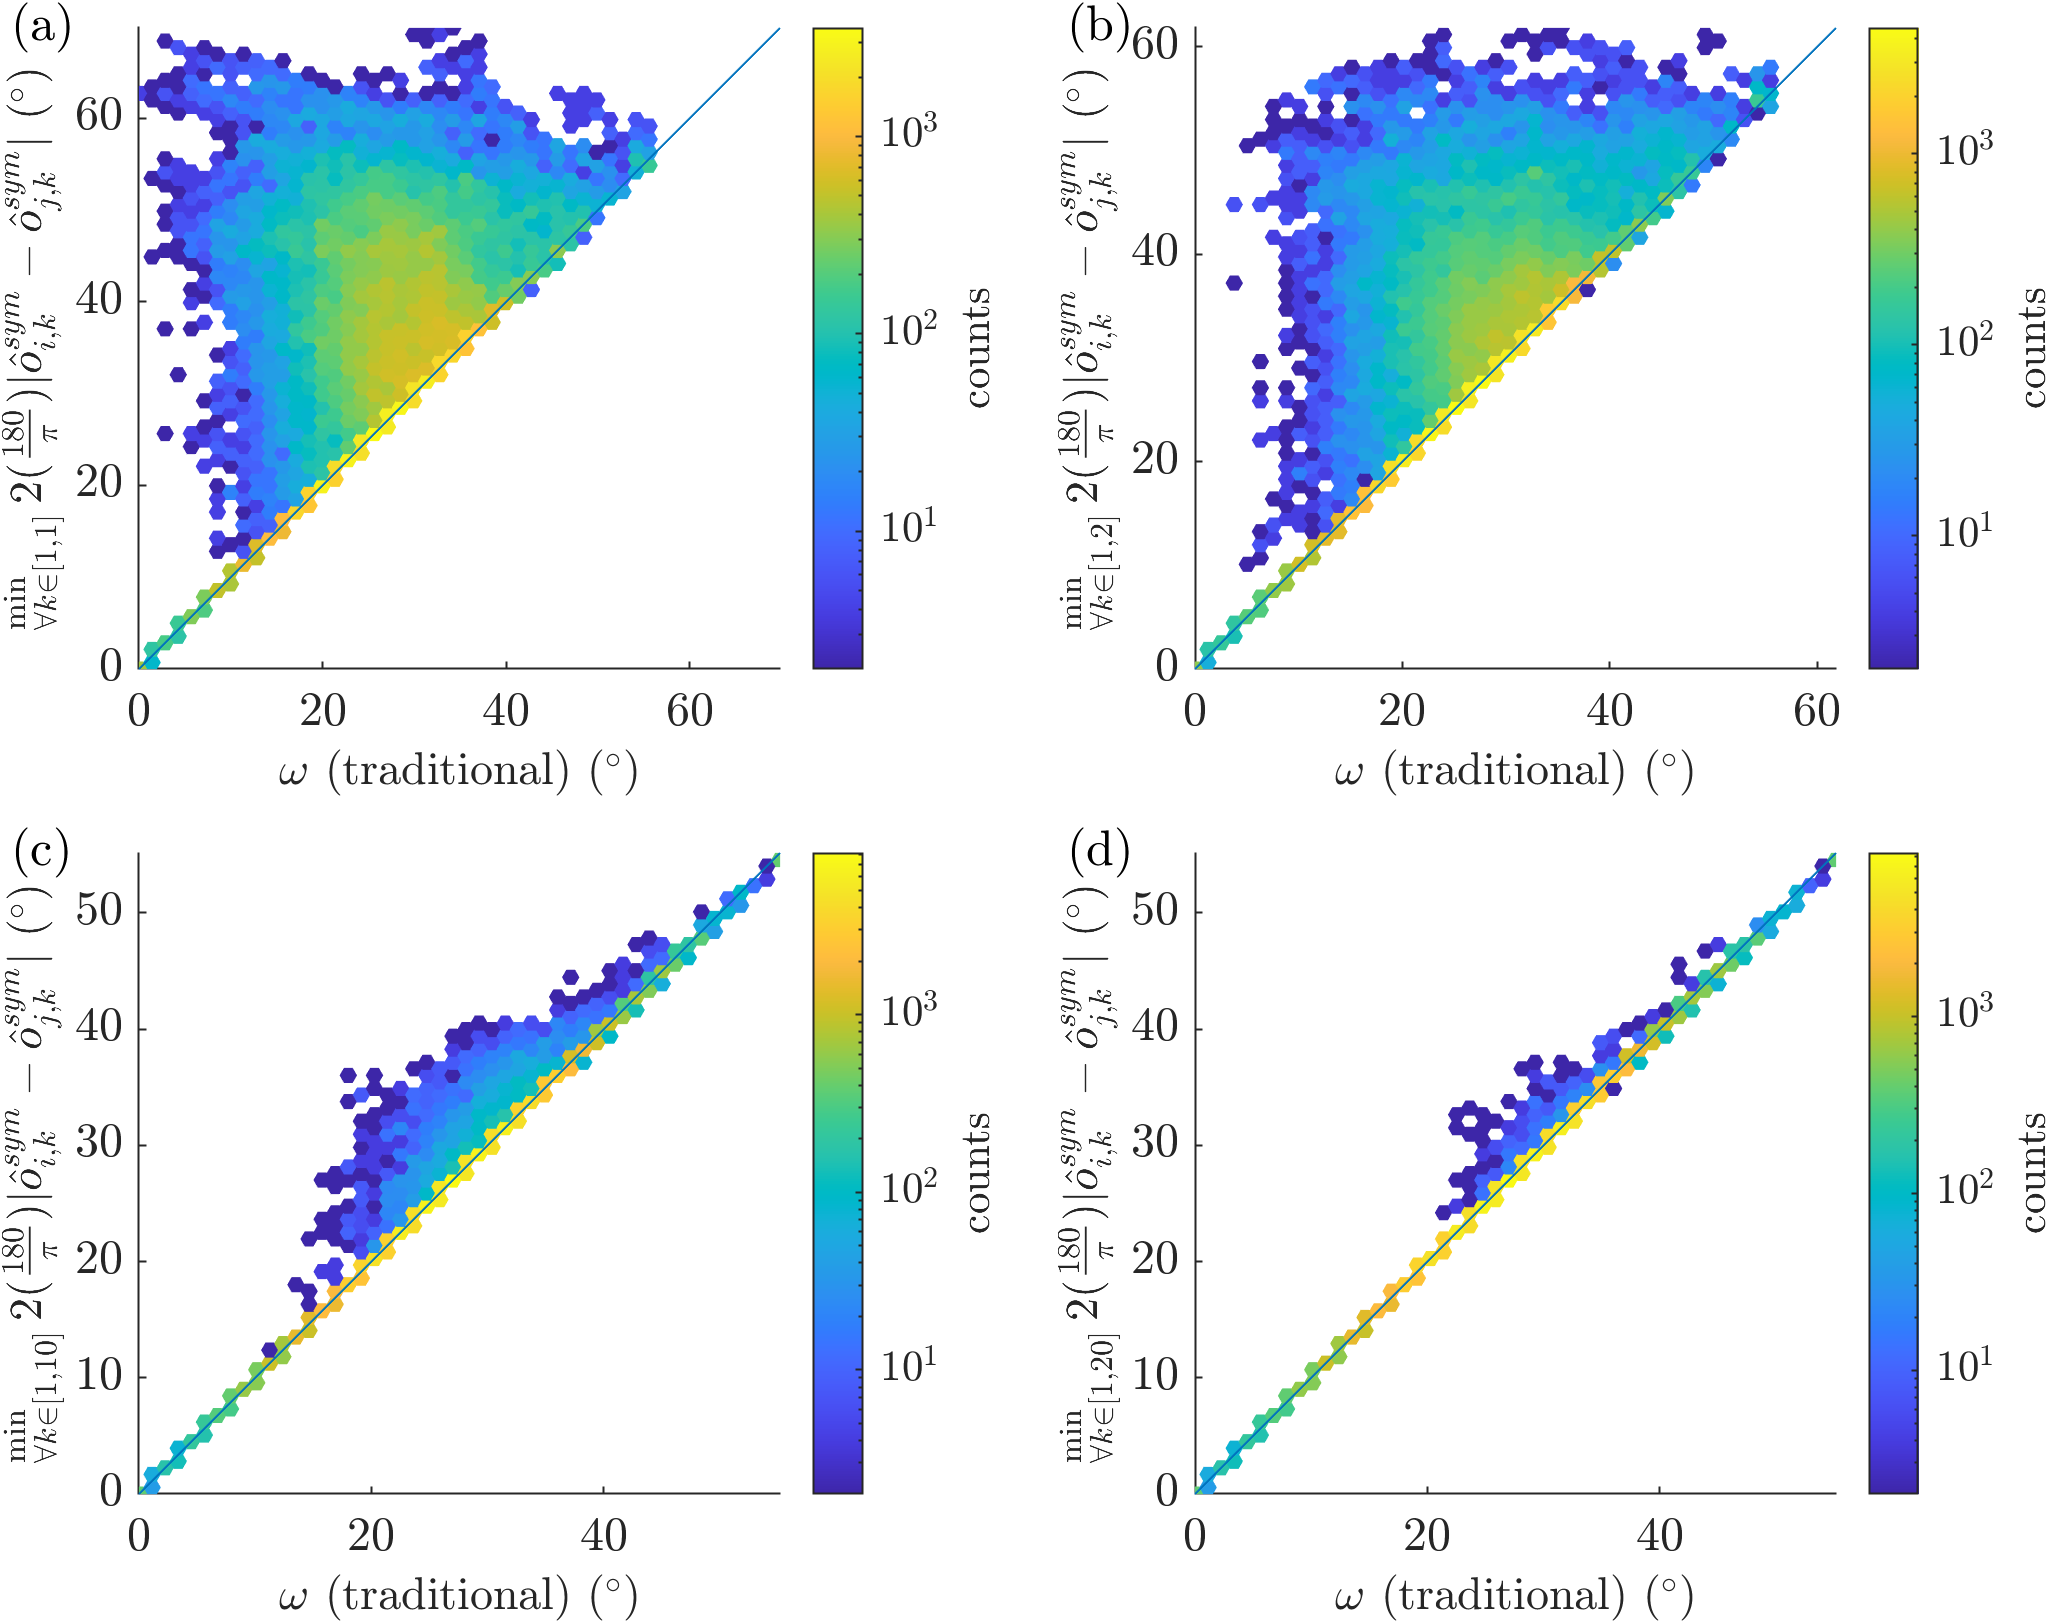
\includegraphics[scale=1]{figures/dist-ensemble-k1-2-10-20.png}
%		\caption{Hexagonally binned parity plots of pairwise distances of 388 Ni bicrystals \cite{olmstedSurveyComputedGrain2009a}. Euclidean distance approximation is converted to \glspl{gbo} ($x_{i,j,k}=2\left(\frac{180}{\pi}\right)|\hat{o}_{i,k}^{\text{sym}}-\hat{o}_{j,k}^{\text{sym}}|$) for comparison with the traditional \gls{gbo} metric \cite{chesserLearningGrainBoundary2020}. The minimum distance among an ensemble of \gls{vfzgbo} sets ($\min_{\forall k \in [1,k_{max}]}x_{i,j,k}$) is used for (a) 1, (b) 2, (c) 10, and (d) 20 \gls{vfzgbo} sets. As the number of \gls{vfzgbo} sets increases, the correlation between the Euclidean distance and the traditional \gls{gbo} distance improves.}
%		\label{fig:dist-ensemble-k1-2-10-20}
%	\end{figure*}
	
	%This is a limitation of the \gls{vfz} framework, which generates a \gls{vfz} with low-symmetry \glspl{gb} at the borders in contrast to typical \glspl{fz} \cite{patalaSymmetriesRepresentationGrain2013,homerGrainBoundaryPlane2015}. While defining a \gls{fz} with high-symmetry \glspl{gb} at the borders (especially mirror-symmetry \glspl{gb}) will certainly increase interpolation accuracy, the favorable interpolation results presented in this work are obtained because overestimation is infrequent within a small correlation length (e.g. \SI{10}{\degree} \cite{olmstedSurveyComputedGrain2009}, which many \glspl{nn} fall within for a \num{50000} \gls{vfzgbo} set, see \cref{fig:nnhist-knn-50000}b), and underestimation is non-existent within numerical precision. Naturally, smaller dataset pairwise distance matrices will exhibit more frequent distance overestimation.
	
	%Overestimation imposes a "sparseness" of data within a local region of influence common to the interpolation methods in this work, whereas underestimation would give erroneous high correlations between uncorrelated \glspl{gb}. Because only overestimation relative to traditional \gls{gbo} distances exist in this work (as shown in \cref{fig:dist-ensemble-k1-2-10-20}), we expect that large errors will occur infrequently (\cref{sec:results:accuracy}). 
	
	%While distance calculations are subject to these infrequent overestimates, they are largely immaterial for interpolation. This is because all interpolation methods in this work involve a region of influence that is small, so that if the distance to a \gls{nn} is overestimated it simply does not contribute to the interpolation (the "sparseness" referred to earlier). Consequently the accuracy of the interpolation is not significantly impacted by infrequent distance overestimates, and excellent results can be achieved without addressing this limitation. However, if even greater accuracy is desired it can be obtained for a relatively minor cost by considering multiple \glspl{vfz}.
	
	%We find that taking the minimum distance among several \gls{vfzgbo} sets defined by separate reference \glspl{gbo} leads to better correlation between the Euclidean approximation and the traditional \gls{gbo} metric as shown in \cref{fig:dist-ensemble-k1-2-10-20}. Additionally, \cref{fig:dist-ensemble-rmse-mae} shows that the error between scaled Euclidean distance and the traditional \gls{gbo} metric decreases rapidly as the number of ensemble \gls{vfzgbo} components increases. This confirms that employing a small ensemble of \gls{vfzgbo} sets results in significant improvement to the Euclidean distance approximation (\cref{fig:dist-ensemble-k1-2-10-20,fig:dist-ensemble-rmse-mae}) of the traditional \gls{gbo} metric. However, as already mentioned, improvements to interpolation results are expected to be less significant since they are already robust to occasional distance overestimates. In terms of computational runtime, use of an ensemble of 10 \glspl{vfz} will increase runtime by a factor of $\sim$10 via a loop-based implementation. For a symmetrized $\num{50000}\times\num{50000}$ pairwise distance matrix, this results in a runtime of approximately 1~CPU~hour instead of $\sim$7 CPU minutes for a single \gls{vfz}. However, this is still much faster than the original \gls{gbo} approach used in \cite{chesserLearningGrainBoundary2020}, which would take an estimated 6.6 CPU years using the original implementation (or 153 CPU days if one \gls{gb} in the \gls{gb} pair is fixed according to the assumption in \citet{morawiecDistancesGrainInterfaces2019}). Additionally, it may be worthwhile to make the distance calculations GPU-compatible for further speed-up. %might be worth making a note here about how many function calls you might expect during a single grain growth simulation. Then we can translate these times into expected minimum CPU time for a 3D grain growth simulation for X number of grains. Maybe Jose has an estimate for this. I think I included something later
%	
%	\begin{figure}[ht]
%		\centering
%		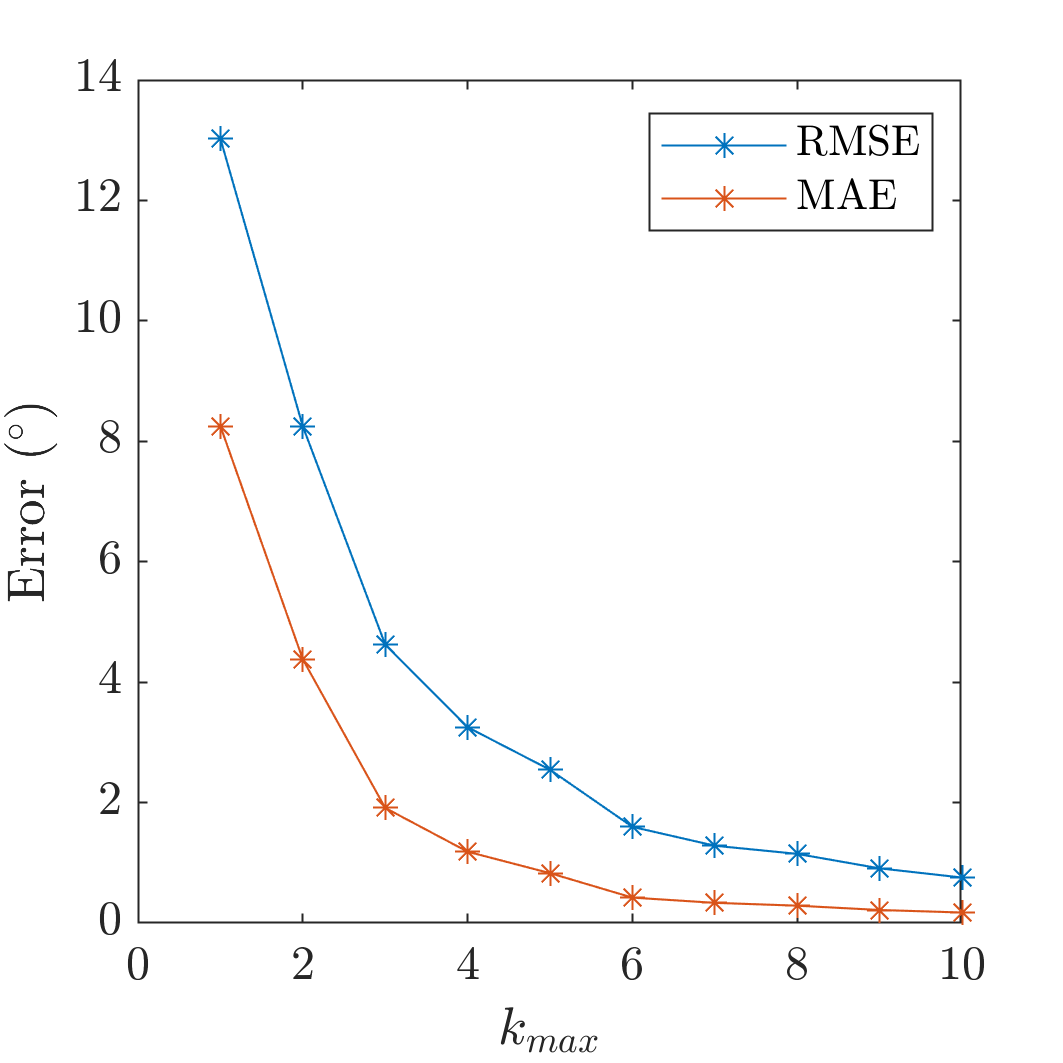
\includegraphics[scale=1]{figures/dist-ensemble-rmse-mae.png}
%		\caption{\Gls{rmse} and \gls{mae} of pairwise distance errors for 388 Ni bicrystals \cite{olmstedSurveyComputedGrain2009} of scaled Euclidean distance approximation relative to the traditional \gls{gbo} metric \cite{chesserLearningGrainBoundary2020} (compare with \cref{fig:dist-ensemble-k1-2-10-20}). The minimum distance among an ensemble of \gls{vfzgbo} sets ($\min_{\forall k \in [1,k_{max}]}x_{i,j,k}$, where $x_{i,j,k}$ is the scaled Euclidean distance) is taken, iteratively adding consecutive sets up to $k_{max} = 20$. As the number of \gls{vfzgbo} sets increases, \gls{rmse} and \gls{mae} between the scaled Euclidean distance approximation and the traditional \gls{gbo} distance decreases.}
%		\label{fig:dist-ensemble-rmse-mae}
%	\end{figure}
	%
	%\Gls{vfzgbo} Euclidean, hyperspherical arc length, and \gls{gbo} distances are computed via \vfzorepo{} function \matlab{GBdist4.m} which is used in the symmetrization function \matlab{get\_octpairs.m} and an example of ensemble \gls{vfzgbo} distance calculations is given in \matlab{plotting.m}.
	%
	%In addition to their use for distance calculations alone, ensembles of \gls{vfzgbo} sets can be employed with interpolation methods to increase overall interpolation accuracy, but there is a computational cost (e.g. approximately 10$\times$ using an ensemble of 10 \gls{vfzgbo} sets). For \num{50000} \inpt{} points, use of an ensemble with 10 \gls{vfzgbo} sets decreases \gls{rmse} and \gls{mae} from \SIlist{0.0241;0.0160}{\J\per\square\m} to \SIlist{0.0187;0.0116}{\J\per\square\m}, respectively (single trial run). We expect these overall accuracy improvements occur because \gls{gbe} predictions near the exterior of the \gls{vfz} where data may be sparse are improved. Ensemble interpolation results as a function of ensemble size and parity plots for mean, median, minimum, and maximum functions applied to the ensemble are shown in \cref{fig:ensemble-interp-rmse-mae} and \cref{fig:ensemble-interp}, respectively. Further details of ensemble interpolation are given in \cref{sec:ensemble-interp}.
	%
% 	\subsection{Interpolation in the \glsentrytitlecase{vfz}{long} Framework} \label{sec:methods:framework:interp}
%	
	Note that in the original definition of the \gls{vfz}, the authors examined different interpolation techniques \cite{bairdFiveDegreeofFreedomPropertyUnderReview}. In the present work, we focus on \gls{gpr} which in our case imposes the assumption that crystallographically similar \glspl{gb} share similar \glspl{gbe} within some correlation length. \Gls{gpr} has the added benefit of built-in uncertainty quantification.
	%With the \gls{vfz} framework established, it is possible to define interpolation schemes over the \gls{vfz} to predict the properties of new \glspl{gb} from the known properties of other \glspl{gb}. For one application of interest to us, it is necessary to evaluate multiple different functions over a fixed set of \inpt{} and \outpt{} \glspl{gbo}. In this section we first present a barycentric interpolation method that we have developed to efficiently accomplish this specialized task by pre-computing the interpolation weights (which remain fixed when only the function being evaluated changes). We then present adaptations of three other interpolation methods---\gls{gpr} (\cref{sec:methods:interp:gpr}), \gls{idw} (\cref{sec:methods:interp:idw}), \gls{nn} (\cref{sec:methods:interp:nn})---that are useful for general applications (an additional interpolation method---\gls{gprm}---which we developed specifically for a non-uniformly distributed, noisy, simulation dataset is described in \cref{sec:methods:gprmix}). %We recommend the \gls{gpr} interpolation method for the \gls{vfz} framework for most applications because it provides the best combination of accuracy and speed (\cref{sec:results}).
	%Usage instructions for the \gls{vfzgbo} repository can be found at the GitHub page (\url{github.com/sgbaird-5dof/interp}) and in \cref{sec:methods:repofn}.
%	
%	
%	\subsubsection{Barycentric Interpolation}
%	\label{sec:methods:interp:bary}
%	
%	Barycentric coordinates are a type of homogeneous coordinate system that reference a \outpt{} point within a simplex \cite{langerSphericalBarycentricCoordinates2006} or convex polytope \cite{floaterGeneralizedBarycentricCoordinates2015,meyerGeneralizedBarycentricCoordinates2002,langerSphericalBarycentricCoordinates2006} based on "masses" or weights at the vertices, which can be negative. The \outpt{} point is assumed to be the barycenter (center of mass) of the simplex or convex polytope, and weights at the vertices necessary to make this assumption true are determined. We utilize rigid \gls{svd} transformations and a standard triangulation algorithm (quickhull \cite{barberQuickhullAlgorithmConvex1996} via \matlab{delaunayn()} in \vfzorepo{} function \matlab{sphconvhulln.m}) to define a simplicial mesh (\cref{sec:app:bary:tri}). We then use barycentric weights (i.e. coordinates) for computing intersections of a point within a simplicial facet (\cref{sec:app:bary:int}) and for interpolation (\cref{sec:app:bary-interp}) \cite{langerSphericalBarycentricCoordinates2006}. A detailed explanation of the process is provided in \cref{sec:app:bary}. %The barycentric interpolation method is invoked in \matlab{interp5DOF.m} by setting the \matlab{method} argument to \matlab{'pbary'}.
%	
%	\subsubsection{\glsentrytitlecase{gpr}{long}}
%	\label{sec:methods:interp:gpr}
%	
%	\Gls{gpr} or Kriging uses the notion of similarity between points to fit Gaussian processes (random variables) to data based on prior information and provides uncertainty information in addition to interpolated or inferred values. For a general treatment of \gls{gpr}, see \citet{rasmussenGaussianProcessesMachine2006}. We use MATLAB's built-in function, \matlab{fitrgp()}, with all default parameters\footnote{MATLAB R2020b was used for the Fe simulation dataset, all other results employed MATLAB R2019b, the latest installed version on our computing cluster.} except that a \gls{fic} approximation is used (\matlab{PredictMethod = 'fic'}) regardless of the number of \inpt{} points. We assume a Euclidean approximation of the \gls{vfz} (see \cref{sec:methods:framework:vfz-dist} and \cref{fig:dist-parity}). A slower, more accurate, and more memory-intensive prediction method that doesn't use sparse approximation (\matlab{PredictMethod = 'exact'}) is also available (\cref{sec:results:efficiency}). %The \gls{gpr} interpolation method is invoked in \matlab{interp5DOF.m} by setting the \matlab{method} argument to \matlab{'gpr'}.
%	
%	\subsubsection{\glsentrytitlecase{idw}{long} Interpolation}
%	\label{sec:methods:interp:idw}
%	
%	\Gls{idw} interpolation applies a weighted average to points within a neighborhood of a query point to obtain an interpolated value. \matlab{interp5DOF.m} implements a simple \gls{idw} approach based on \cite{tovarInverseDistanceWeight2020}. A default radius of influence of $r=\sqrt{2} \mu$ is used, where $\mu$ represents the mean \gls{nn} distance, and where \gls{gbo} distance is approximated by the Euclidean distance or 2-norm (see \cref{sec:methods:framework:vfz-dist}, and \cref{fig:dist-parity}). \gls{nn} interpolation (\cref{sec:methods:interp:nn}) is used for a given query point when there are no \inpt{} points in the radius of influence. %The \gls{idw} interpolation method is invoked in \matlab{interp5DOF.m} by setting the \matlab{method} argument to \matlab{'idw'}.
%	
%	\subsubsection{\glsentrytitlecase{nn}{long} Interpolation}
%	\label{sec:methods:interp:nn}
%	
%	\Gls{nn} interpolation takes the nearest \inpt{} point relative to a query point and assigns the value of the \gls{nn} \inpt{} point to the query point. This is implemented via the built-in MATLAB function \matlab{dsearchn()} using a Euclidean approximation of \gls{gbo} distance (see \cref{sec:methods:framework:vfz-dist}, and \cref{fig:dist-parity}). %The \gls{nn} interpolation method is invoked in \matlab{interp5DOF.m} by setting the \matlab{method} argument to \matlab{'nn'}.
%	
%	
% 	\subsection{Comparison with Traditional \glsentrytitlecase{gbo}{short} Framework} \label{sec:methods:framework:compare}
%
	The primary differences between the \gls{vfz} framework and traditional \gls{gbo} distance metric are that the \gls{vfz} framework is defined by a continuous set of points, exhibits occasional distance overestimation, uses a Euclidean approximation, and has a lower computational complexity.
%	We compare the \gls{vfz} framework with the traditional \gls{gbo} metric (\cref{tab:closed-mesh-comparison}) and give examples that illustrate the computational complexity of each approach.
	
%	\begin{table*}
%		\caption{Comparison between \glsxtrlong{vfzgbo} and traditional \gls{gbo} frameworks. *6D Cartesian representation used only for mesh triangulation efficiency in barycentric interpolation and *7D Cartesian representation only required for barycentric interpolation. 7D Cartesian representation is also implemented (though not required) for \gls{gpr}, \gls{nn}, and \gls{idw}. For pairwise distance complexity, $N_p$ is the number of proper rotations ($N_p=24$ for $m\Bar{3}m$ \gls{fcc} point group) and $L$ is the number of \glspl{gb}.}
%		\centering
%		\begin{tabular}{ccc}
%			\toprule
%			Property & Traditional & This Work \\
%			\midrule
%			Symmetrizing Distance & \gls{gbo} & \gls{vfz} Euclidean \\
%			% Considered \glspl{seo} & Subset & All \\
%			Dimensionality & 8D Cartesian & 6*/7*/8D Cartesian \\
%			Bounded by \gls{fz} & No & Yes \\
%			% Euclidean Approximation Valid & No & Yes \\
%			Pairwise Distance Complexity & $O(N_p^2L^2)$ & $O(N_p^2L)$ \\
%			Rotation Convention & Passive & Active \\
%			\bottomrule
%		\end{tabular}
%		\label{tab:closed-mesh-comparison}
%	\end{table*}
	
	%The construction of the \gls{vfz} dramatically reduces the computational burden of pairwise distance calculations. The mechanism by which this reduction is achieved can be illustrated with an example. Let $o_1$ and $o_2$ denote two \glspl{gb} represented in \gls{gbo} coordinates. 
	%To perform a traditional symmetrized \gls{gbo} distance calculation according to \citet{francisGeodesicOctonionMetric2019}, we compare all \glspl{seo} of $o_1$ to all of the \glspl{seo} of $o_2$ and take the smallest distance. If $N_p$ is the number of proper rotations of the crystallographic point group, this single minimum distance calculation requires a total of $4N_p^4$ \glspl{seo} to be considered (Sections 4.3 and 4.5 of \citet{francisGeodesicOctonionMetric2019}). Thus, the total number of \gls{seo} computations will be $4N_p^4L^2$. However, it is possible to fix a single \gls{gb} in the \gls{gb} pair and still obtain accurate\footnote{Compared with the pairwise distance matrix of the 388 Olmsted \glspl{gb}, we obtained a \gls{rmse} of \SI{1.6566E-7}{\degree} for this computation which completed in \SI{133}{\s} using 6 cores (see \matlab{get_pd_fix.m})} due to isometry equivalence (see Section 7 of \cite{morawiecDistancesGrainInterfaces2019} and \cref{fig:pd-fix}).
%	
%	In contrast, for a single distance calculation using the \gls{vfz} framework, $o_1$ and $o_2$ are first mapped into the \gls{vfz}, and then only a single distance calculation is required between them. Mapping $o_1$ into the \gls{vfz} requires comparison of $8N_p^2$ \glspl{seo}\footnote{This is 8 instead of 4 because the simplifying assumption that only two of the four double cover cases need to be considered \cite{francisGeodesicOctonionMetric2019} does not apply in the \gls{vfz} framework. This is confirmed by applying \matlab{uniquetol()} on a set of $4608$ \glspl{gbo} which has a final set size of $4608$, where $4608=8\times N_p^2$ and $N_p=24$ (see \matlab{osymset.m}).} of $o_1$ with a fixed reference \gls{gb} in the interior of the \gls{vfz}; and likewise for $o_2$. Consequently, a single distance calculation between $o_1$ and $o_2$ under the \gls{vfz} framework requires $O(N_p^2)$ \gls{seo} computations. If one desires to compute a pairwise distance matrix between $L$ \glspl{gb}, the total computational cost\footnote{See \cref{sec:results:efficiency:symruntime} for a detailed explanation of why this is \emph{not} $O(N_p^2L^2)$.} will be $O(N_p^2L)$, which represents a dramatic reduction compared to the traditional approach. A summary of the differences between the two approaches is provided in \cref{tab:closed-mesh-comparison}.
	
% 	\subsection{Generating Random \glsentrytitlecase{vfzgbo}{long}s}
% 	\label{sec:methods:rand}
% 	We generate a random \gls{gbo} by sampling a misorientation via a cubochoric approach \cite{singhOrientationSamplingDictionarybased2016}, sampling \gls{bp} normal from the 2-sphere, and converting to these \gls{5dof} coordinates to \gls{gbo} coordinates. %: we pair two cubochorically sampled \glspl{gb} to form a \gls{gbo}.
%	In addition to the 3 core operations of the \gls{vfz} framework described in \cref{sec:methods:framework}, it will be necessary for our tests, and useful for other applications, to be able to generate random \glspl{gbo} from \gls{5dof} representations. We briefly explain here our process for accomplishing this. 
%	
%	First, random \glspl{gbo} are formed by taking random misorientation quaternion (\matlab{qm}) and \gls{bp} normal (\matlab{nA}) pairs. Random misorientation quaternions are obtained via cubochoric sampling \cite{singhOrientationSamplingDictionarybased2016} (\matlab{get\_cubo.m}) and random \gls{bp} vectors are sampled from a multivariate Gaussian distribution ($\mu=0$, $\sigma=1$) in $\mathbb{R}^3$ and normalized\footnote{Several methods for uniform sampling of points on a sphere, including the one mentioned here, are described in \url{https://mathworld.wolfram.com/SpherePointPicking.html}.}. After this, they are converted to \glspl{gbo} via \vfzorepo{} function \matlab{five2oct.m}. The \vfzorepo{} function \matlab{get\_five.m} returns the result of these several operations. These (\matlab{qm},\matlab{nA}) pairs are then converted to an \gls{gbo} representation, \matlab{o}, using \vfzorepo{} function \matlab{o=five2oct(qm,nA)} (see also \vfzorepo{} function \matlab{get\_ocubo.m} for generating random \glspl{gbo} directly).
	%}a modified version \cite{bairdFiveDegreeofFreedom5DOF2020} of the original \matlab{GBfive2oct.m} function \cite{chesserGBOctonionCode2019} via
%	
%	The \glspl{gbo} are then symmetrized (i.e. they become \glspl{vfzgbo}) via \matlab{osym=get\_octpairs(o)}. A default reference \gls{gbo}\footnote{This is generated by \matlab{get\_ocubo.m} using a random number generator seed of 10. We expect that \matlab{five2oct.m} combined with \matlab{get\_five.m} will generate near identical statistical properties to \matlab{get\_ocubo.m} which is supported by a visual comparison of pairwise distance histograms (not shown in this work), and indirectly by an assertion in Section 5.3 of \citet{morawiecDistancesGrainInterfaces2019}. } is used for these calculations, unless specified by the user. We use the active convention for \matlab{qm}, \matlab{nA}, and \matlab{o} (see \cref{sec:app:convention} for further details of conventions).
%	
%	For the present work we use this procedure to randomly generate \gls{vfzgbo} sets containing between \num{100} to \num{50000} \glspl{vfzgbo} where each trial run has its own unique set of \glspl{gb}. We use these to perform the validation and performance evaluation tests described later. For reference, we note that the average \gls{nn} distance (over approximately 70 trials) of such sets ranges between \SI{10.7175 \pm 0.3684}{\degree} and \SI{2.6479 \pm 0.2254}{\degree}, respectively. 

\section{Fe Input Data Quality}
	\label{sec:supp:kim-interp:quality}
	Of the $\sim$\num{60000} \glspl{gb}\footnote{The "no-boundary" \glspl{gb} (i.e. \glspl{gb} with close to \SI{0}{\joule\per\square\meter} \gls{gbe}) were removed before testing for degeneracy.} in \cite{kimPhasefieldModeling3D2014}, $\sim$\num{10000} \glspl{gb} were repeats that were identified by converting to \glspl{vfzgbo} and applying \vfzorepo{} function \texttt{avg\_repeats.m}. In \cite{kimPhasefieldModeling3D2014}, mechanically selected \glspl{gb} were those which involved sampling in equally spaced increments\footnote{In some cases, this was equally spaced increments of the argument of a trigonometric function.} for each \gls{5dof} parameter, and a few thousand intentionally selected \glspl{gb} (i.e. special \glspl{gb}) were also considered. Of mechanically and intentionally selected \glspl{gb}, \numlist{9170;112} are repeats, respectively, with a total of \num{2496} degenerate sets\footnote{A degenerate "set" is distinct from a \gls{vfzgbo} "set", the latter of which is often used in the main text.} (see \cref{fig:kim-interp-degeneracy-sets} for a degeneracy histogram). Thus, on average there is a degeneracy of approximately four per set of degenerate \glspl{gb}.
	
	By comparing \gls{gbe} values of (unintentionally\footnote{To our knowledge, the presence of repeat \glspl{gb} were not mentioned in \cite{kimPhasefieldModeling3D2014} or \cite{kimIdentificationSchemeGrain2011}}) repeated \glspl{gb} in the Fe simulation dataset \cite{kimPhasefieldModeling3D2014}, we can estimate the intrinsic error of the \inpt{} data. For example, minimum and maximum deviations from the average value of a degenerate set are \SIlist{-0.2625;0.2625}{\joule\per\square\meter}, respectively, indicating that a repeated Fe \gls{gb} simulation from \cite{kimPhasefieldModeling3D2014} can vary by as much as \SI{0.525}{\joule\per\square\meter}, though rare. Additionally, \Gls{rmse} and \gls{mae} values can be obtained within each degenerate set by comparing against the set mean. Overall \gls{rmse} and \gls{mae} are then obtained by averaging and weighting by the number of \glspl{gb} in each degenerate set. Following this procedure, we obtain an average set-wise \gls{rmse} and \gls{mae} of \SIlist{0.06529;0.06190}{\joule\per\square\meter}, respectively, which is an approximate measure of the intrinsic error of the data. \cref{fig:kim-interp-degeneracy-results} shows histograms and parity plots of the intrinsic error. The overestimation of intrinsic error mentioned in the main text (\cref{sec:results:lit:error}) could stem from bias as to what type of \glspl{gb} exhibit repeats based on the sampling scheme used in \cite{kimPhasefieldModeling3D2014} and/or that many of the degenerate sets contain a low number of repeats (\cref{fig:kim-interp-degeneracy-sets}).
	
	Next, we see that by binning \glspl{gb} into degenerate sets, most degenerate sets have a degeneracy of fewer than 5 \cref{fig:kim-interp-degeneracy-sets}. We split the repeated data into sets with a degeneracy of fewer than 5 and greater than or equal to 5 and plot the errors (relative to the respective set mean) in both histogram form (\cref{fig:kim-interp-degeneracy-results}a and \cref{fig:kim-interp-degeneracy-results}c, respectively) and as hexagonally-binned parity plots (\cref{fig:kim-interp-degeneracy-results}b and \cref{fig:kim-interp-degeneracy-results}d, respectively). While heavily repeated \glspl{gb} tend to give similar results, occasionally repeated \glspl{gb} often have larger \gls{gbe} variability. This could have physical meaning: Certain types of (e.g. high-symmetry) \glspl{gb} tend to have less variation (i.e. fewer and/or more tightly distributed metastable states). However, it could also be an artifact of the simulation setup that produced this data (e.g. deterministic simulation output for certain types of \glspl{gb}).
	
	\begin{figure}
		\centering
		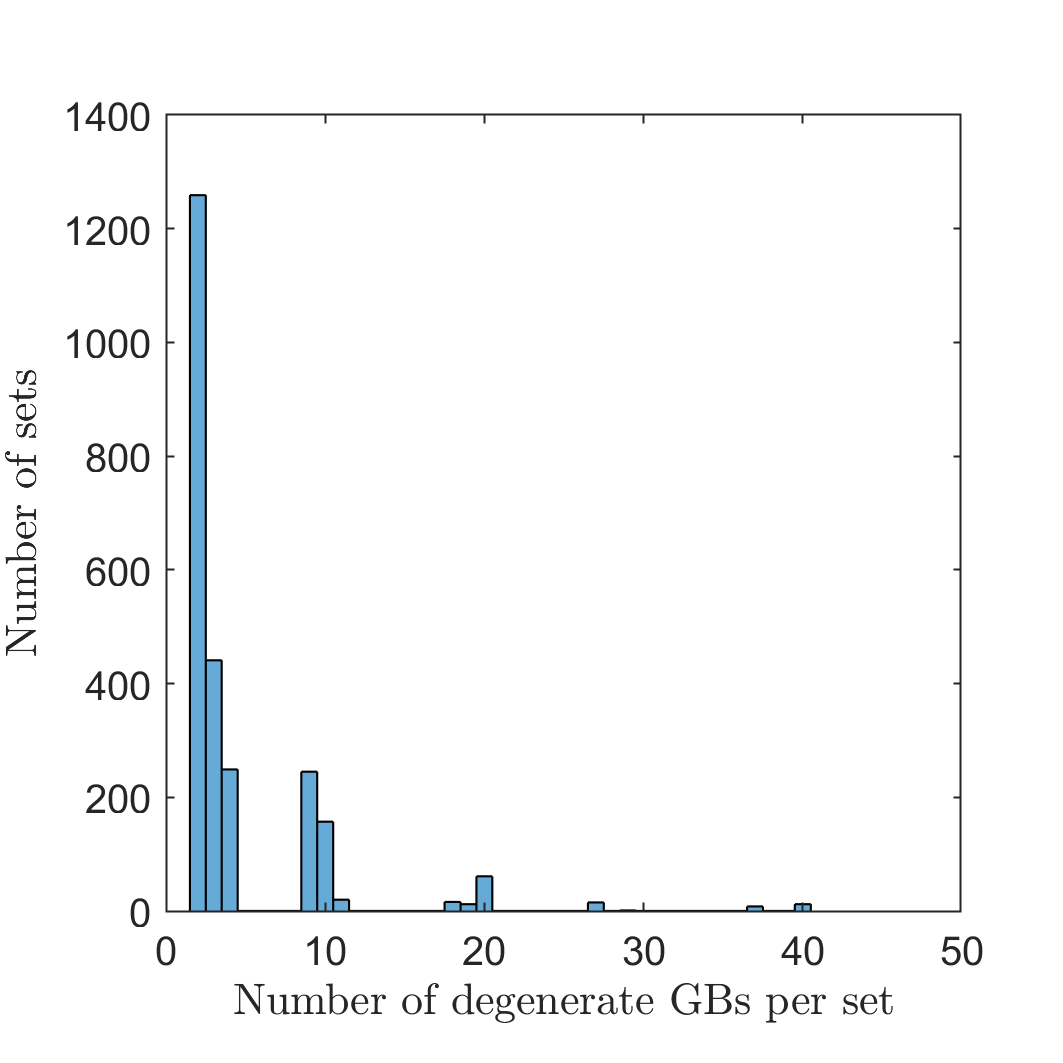
\includegraphics[scale=1]{kim-interp-degeneracy-sets.png}
		\caption{Histogram of number of sets vs. number of degenerate \glspl{gb} per set for the Fe simulation dataset \cite{kimPhasefieldModeling3D2014}. Most sets have a degeneracy of fewer than 5.}
		\label{fig:kim-interp-degeneracy-sets}
	\end{figure}
	
	\begin{figure}
		\centering
		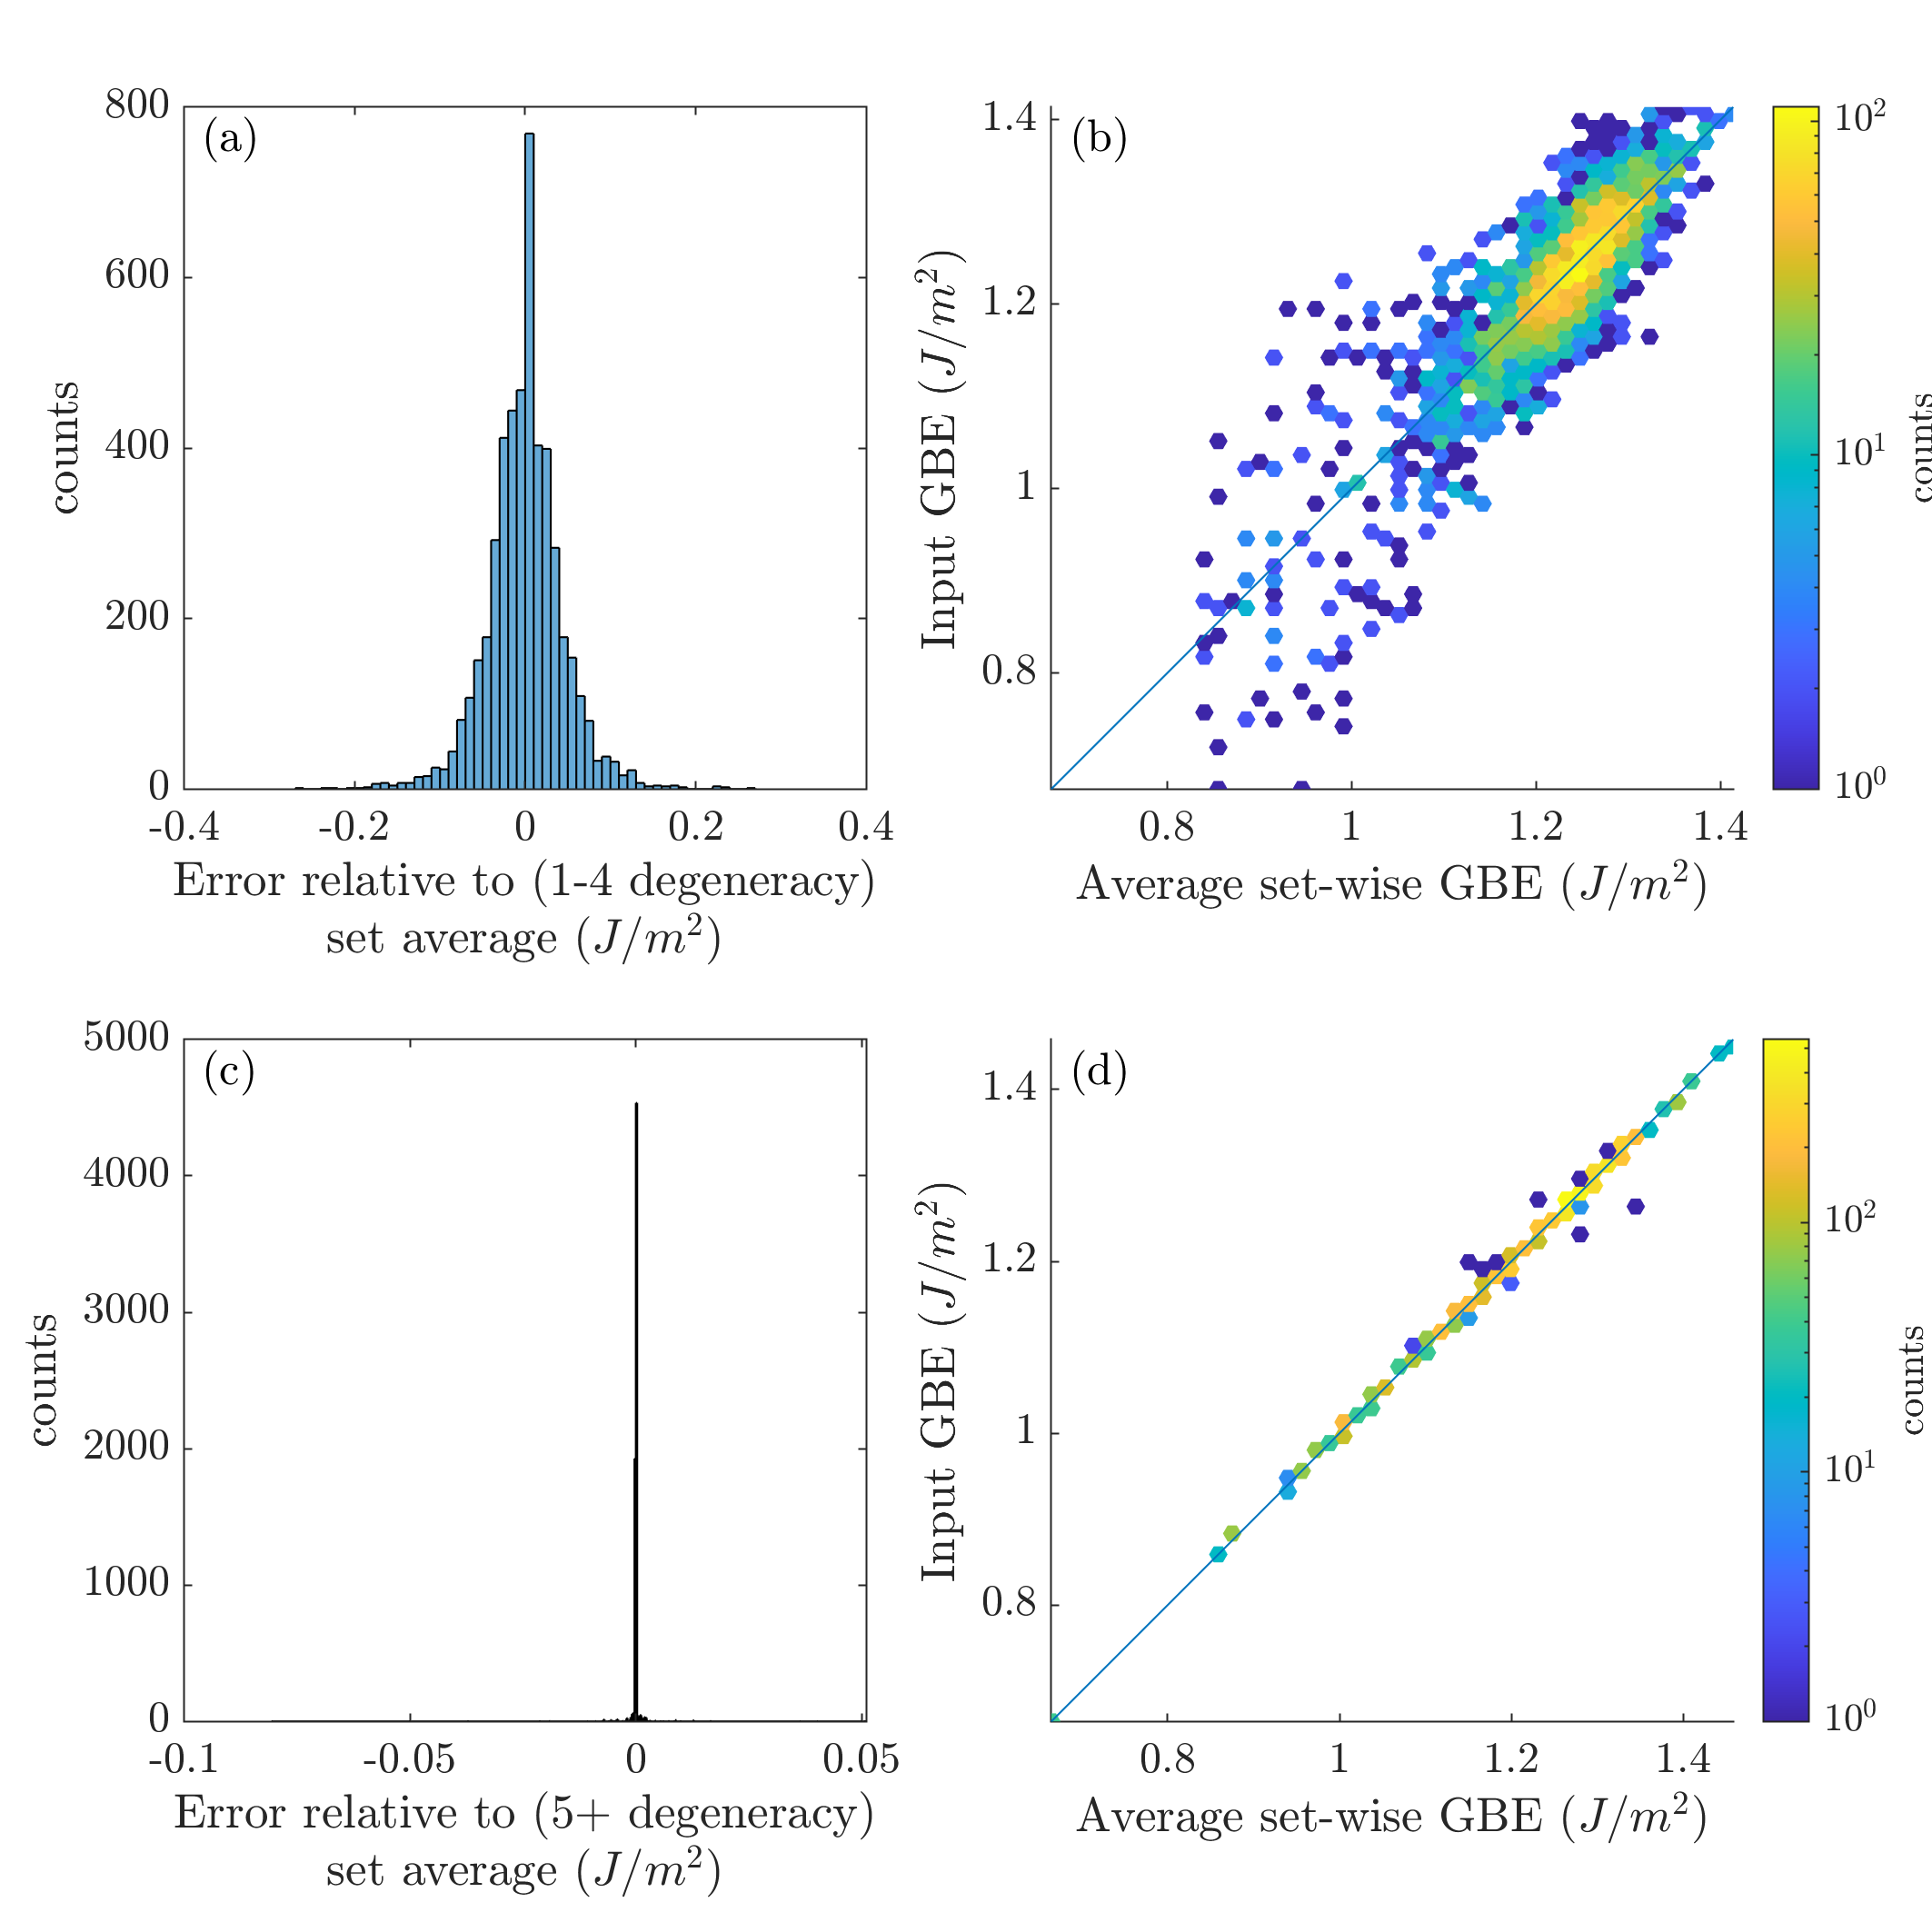
\includegraphics[scale=1]{kim-interp-degeneracy-results.png}
		\caption{Degenerate \glspl{gb} sets are split into those with a degeneracy of fewer than 5 and greater than or equal to 5 and plotted as ( (a) and (c), respectively) error histograms and ( (b) and (d), respectively) hexagonally-binned parity plots. Large degenerate sets tend to have very low error, whereas small degenerate sets tend to have higher error. In other words, \glspl{gb} that are more likely to be repeated many times based on the sampling scheme in \cite{kimPhasefieldModeling3D2014} tend to give similar results, whereas \glspl{gb} that are less likely to be repeated often have larger variability in the simulation output. We do not know if this has physical meaning or is an artifact of the simulation setup.}
		\label{fig:kim-interp-degeneracy-results}
	\end{figure}
	
	% \subsection{Uncertainty Quantification and the Posterior Distribution of \glsentrytitlecase{gprm}{long} }
	% The use of \gls{gpr} in the \gls{gprm} model facilitates uncertainty quantification which we discuss in more detail. We find that use of \cref{eq:gprmix-sigma} on two models with differing amounts of data leads to a model with typically higher uncertainty for low \glspl{gbe} than high \glspl{gbe} (\cref{fig:kim-interp-posterior}a). By observing the \glspl{nn} relative to an arc $\overline{AB}$, we find that there is a large scatter of \glspl{gbe} for \glspl{gb} that are within a radius of $\sim$\SI{6}{\degree} (\cref{fig:kim-interp-posterior}b). By sampling from the posterior distribution, we find that 
	
	% Uncertainty results, as well as posterior samples of the \gls{gprm} distribution of models are shown in \cref{fig:kim-interp-posterior}.
	
	% \begin{figure}
	%     \centering
	%     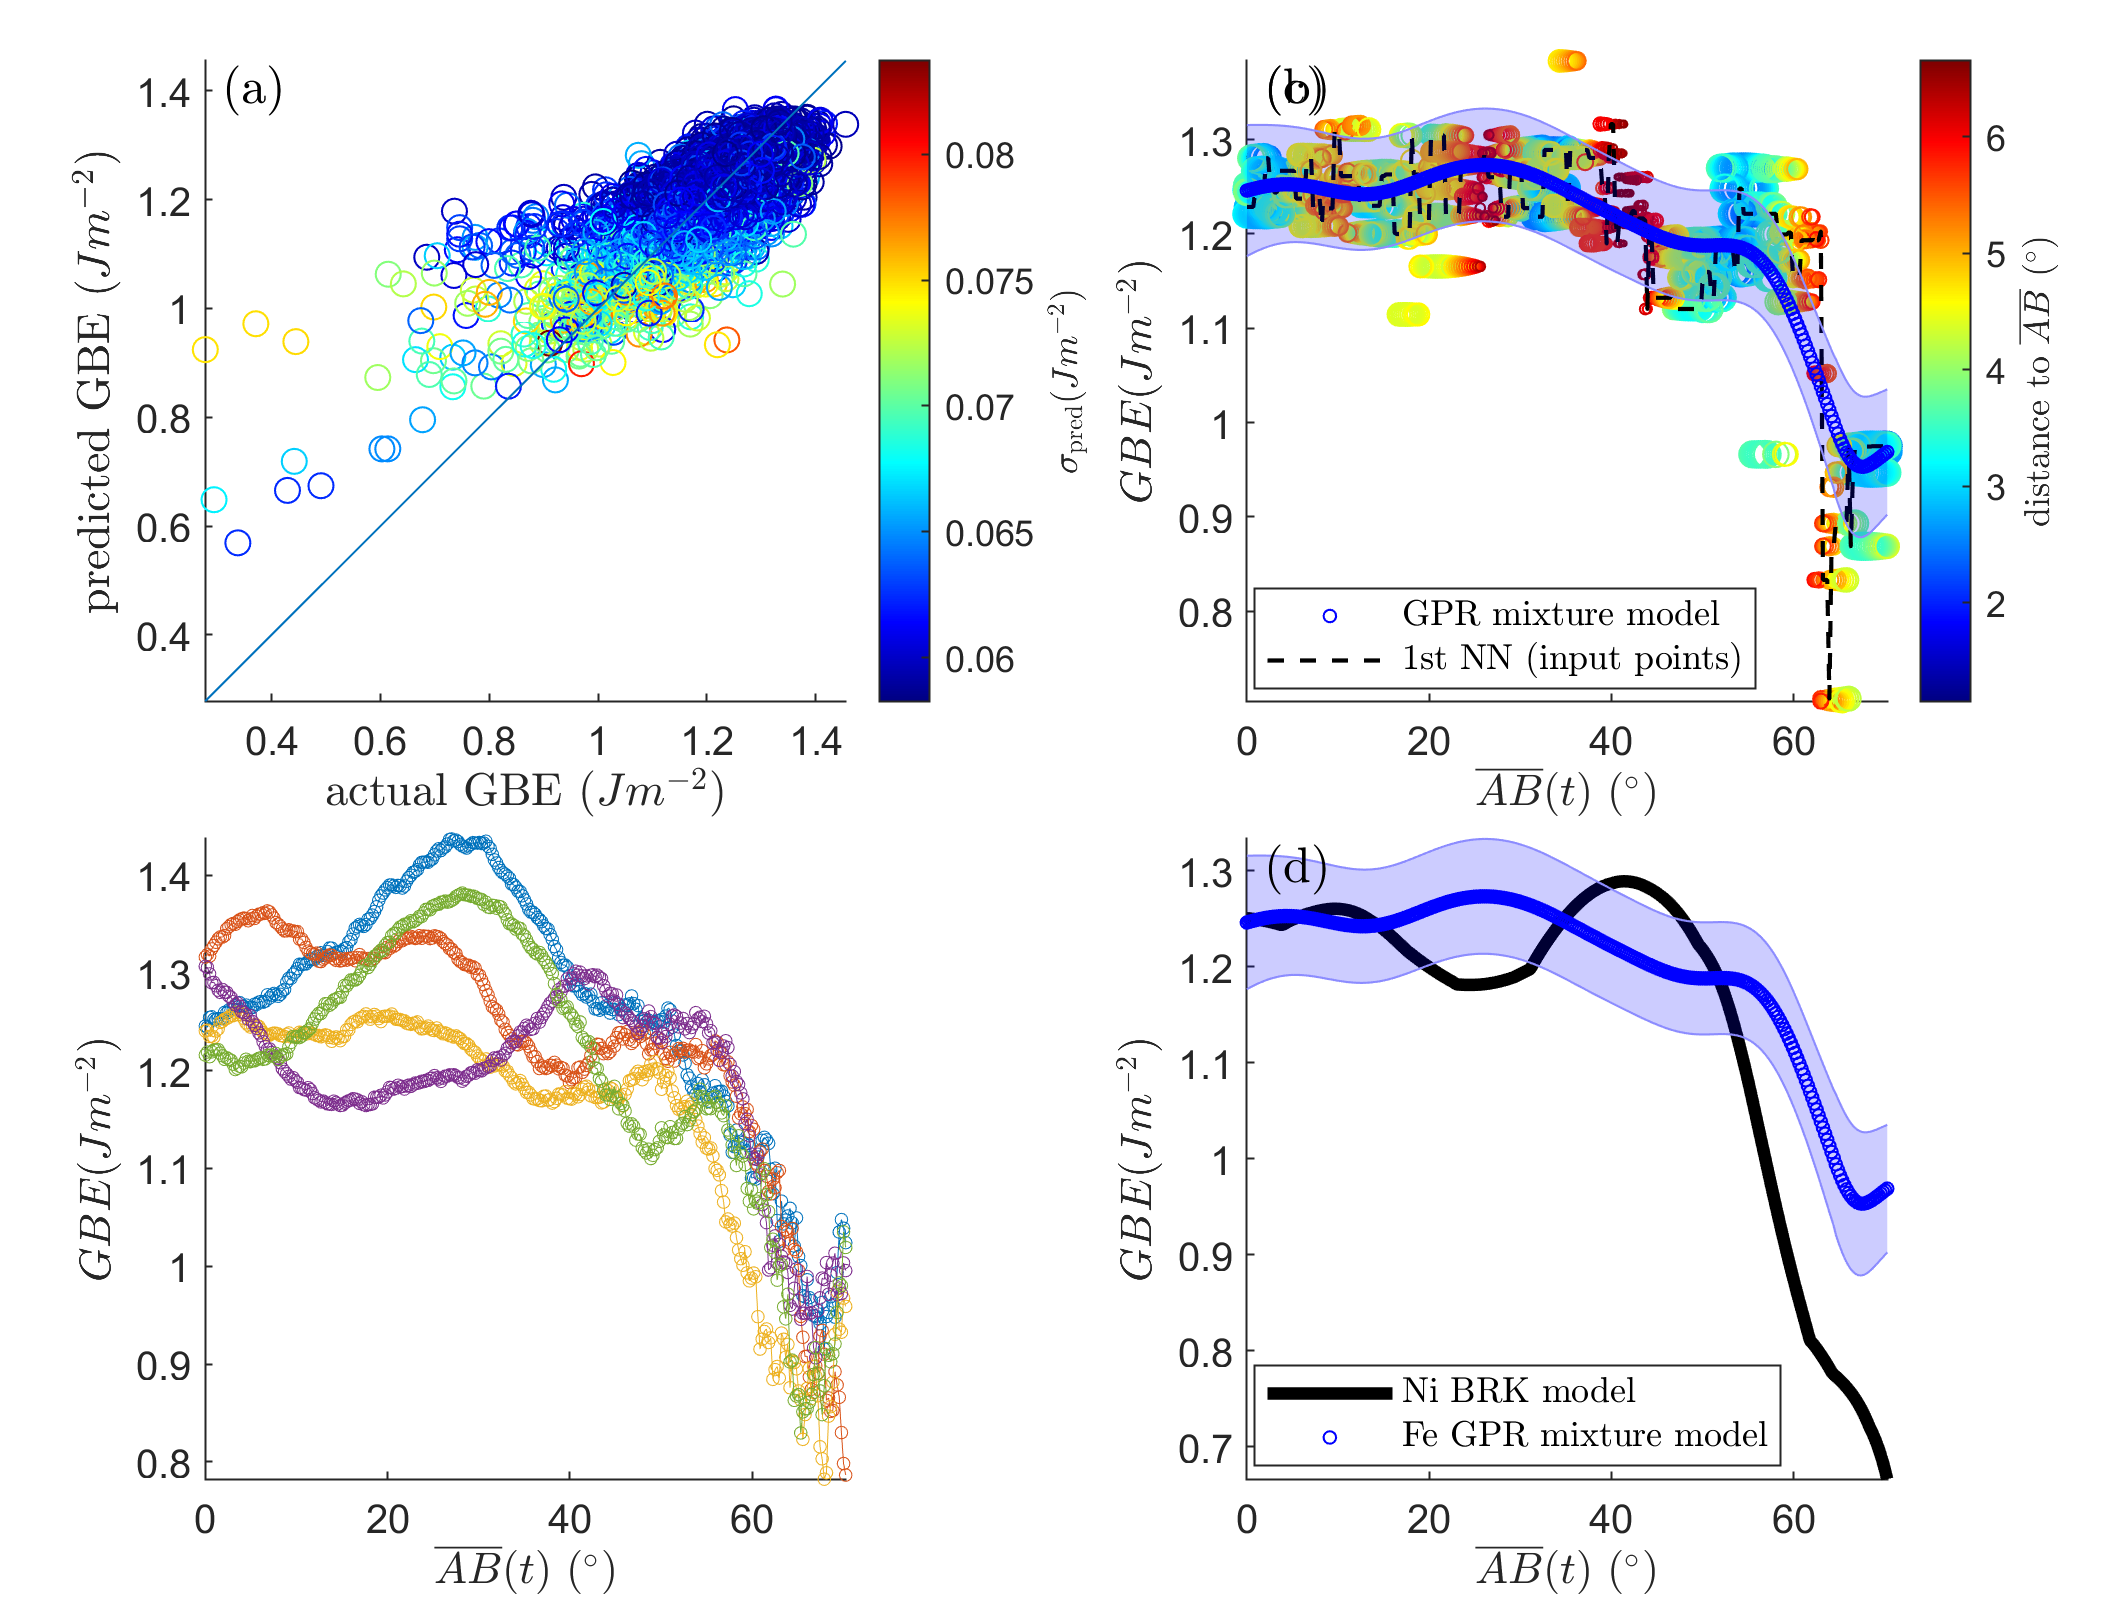
\includegraphics[scale=1]{figures/kim-interp-posterior.png}
	%     \caption{Interpolation results for a large Fe simulation database \cite{kimPhasefieldModeling3D2014} using \num{46883} \inpt{} \glspl{gb} and \num{11721} \outpt{} \glspl{gb} in an 80\%/20\% split and a \gls{gpr} mixture model to better approximate low \glspl{gbe}. (a) Parity plot colored by uncertainty standard deviation. (b) Prediction (black) and uncertainty standard deviation (grey band) of \gls{gpr} mixture model as a function of distance along a 1D arc ($\overline{AB}$) between two \glspl{vfzgbo} ($A$ and $B$). The first \inpt{} \gls{nn} is shown as a black, dashed line. The \inpt{} point \glspl{knn} ($k\in[1,2,3,4,5,6]$) relative to $\overline{AB}$ are colored and sized according to the distance to $\overline{AB}$ (\inpt{} points far from the line are small, dark red circles and \inpt{} points close to the line are large, dark blue circles). In other words, this shows the data in a small region of influence around $\overline{AB}$ that contributed to the model predictions where close data is emphasized (larger) than far-away data (smaller). (c)
	%     Five models sampled from the posterior distribution of the \gls{gpr} mixture model. (d) Fe \gls{gpr} mixture model results and uncertainty standard deviation (grey band) overlaid with the Ni \gls{brk} model along the arc $\overline{AB}$. Coordinates for $A$ and $B$ are given in \cref{tab:tunnel-AB2} of the main paper and 300 equally spaced points are plotted for (b), (c), and (d).}
	%     \label{fig:kim-interp-posterior}
	% \end{figure}

% \section{Tunnel Plots} \label{sec:supp:tunnel}

% 	\begin{figure*}[!htb]
% 		\centering
% 		\begin{subfigure}[b]{0.48\textwidth}
% 			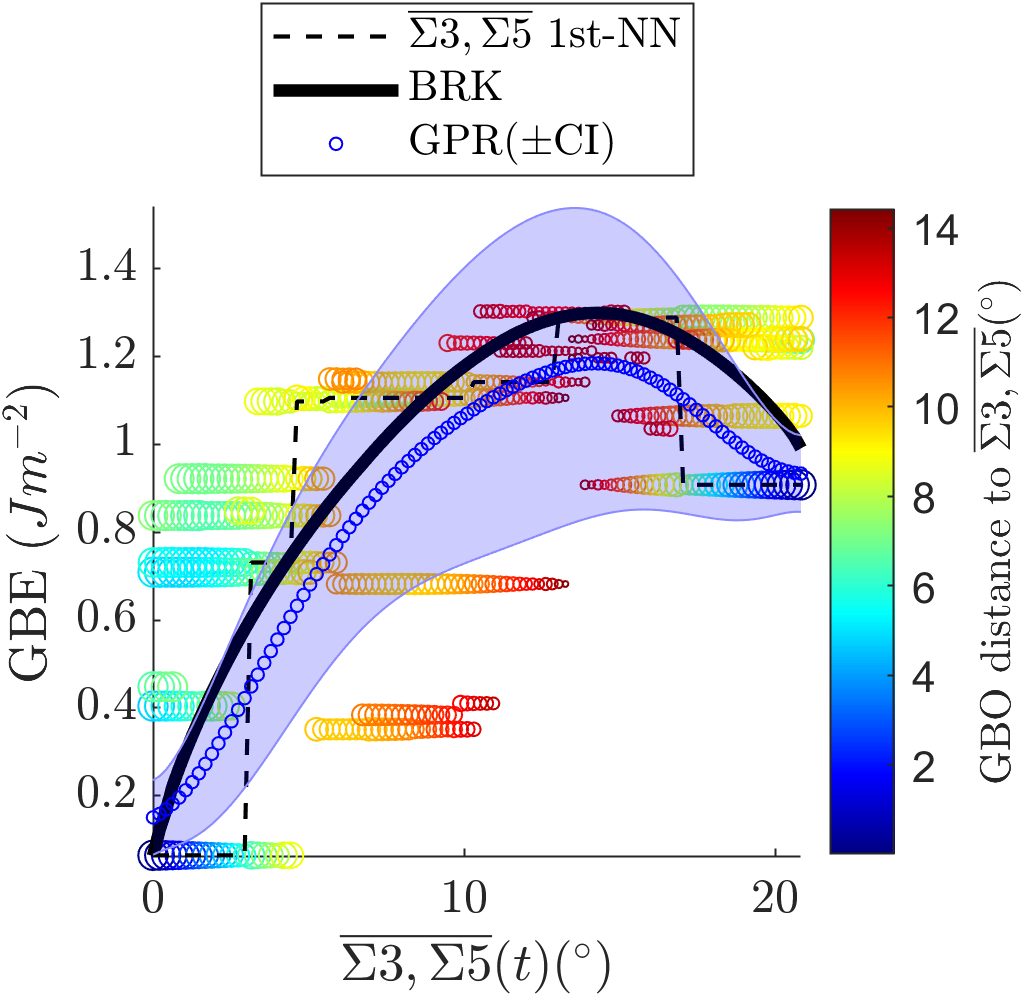
\includegraphics[width=\textwidth]{figures/tunnel-3-5-olmsted.png}
% 			\caption{}
% 			\label{fig:tunnel-3-5-olmsted}
% 		\end{subfigure}
% 		\hfill
% 		\begin{subfigure}[b]{0.48\textwidth}
% 			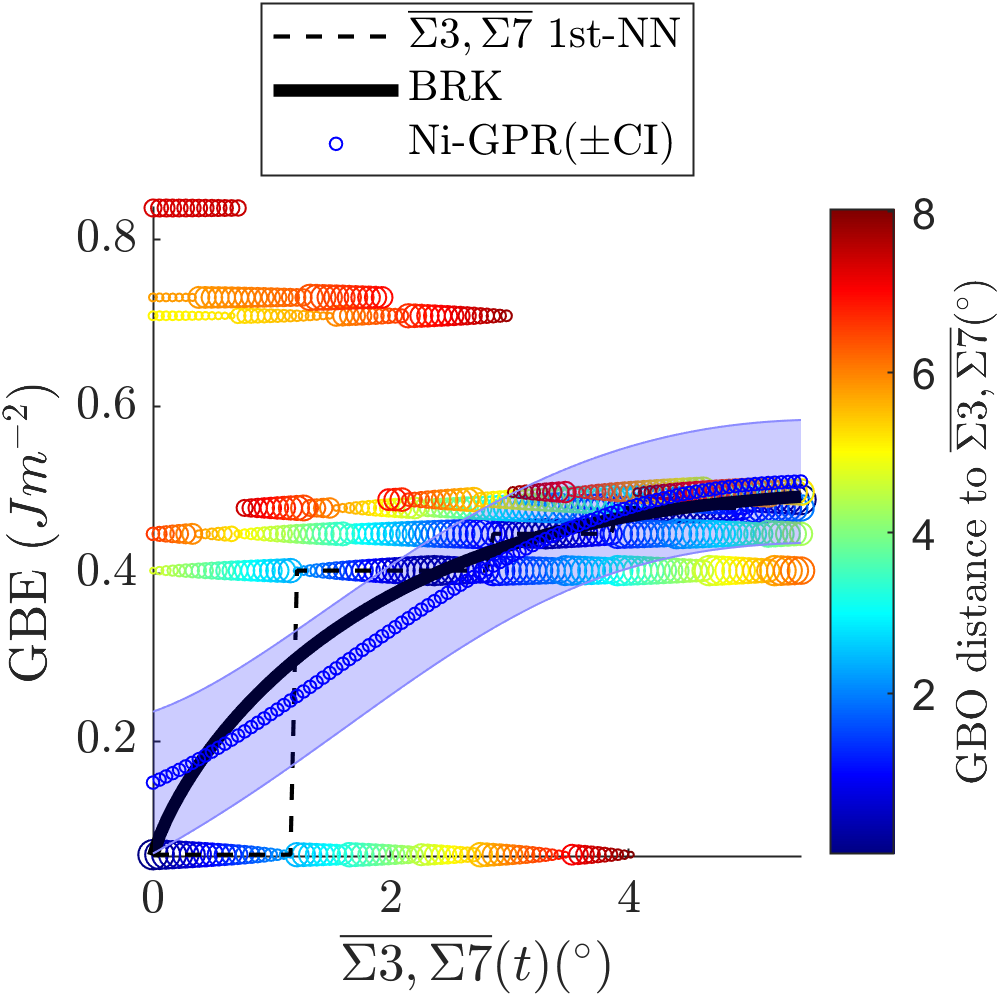
\includegraphics[width=\textwidth]{figures/tunnel-3-7-olmsted.png}
% 			\caption{}
% 			\label{fig:tunnel-3-7-olmsted}
% 		\end{subfigure}
		
% 		\begin{subfigure}[b]{0.48\textwidth}
% 			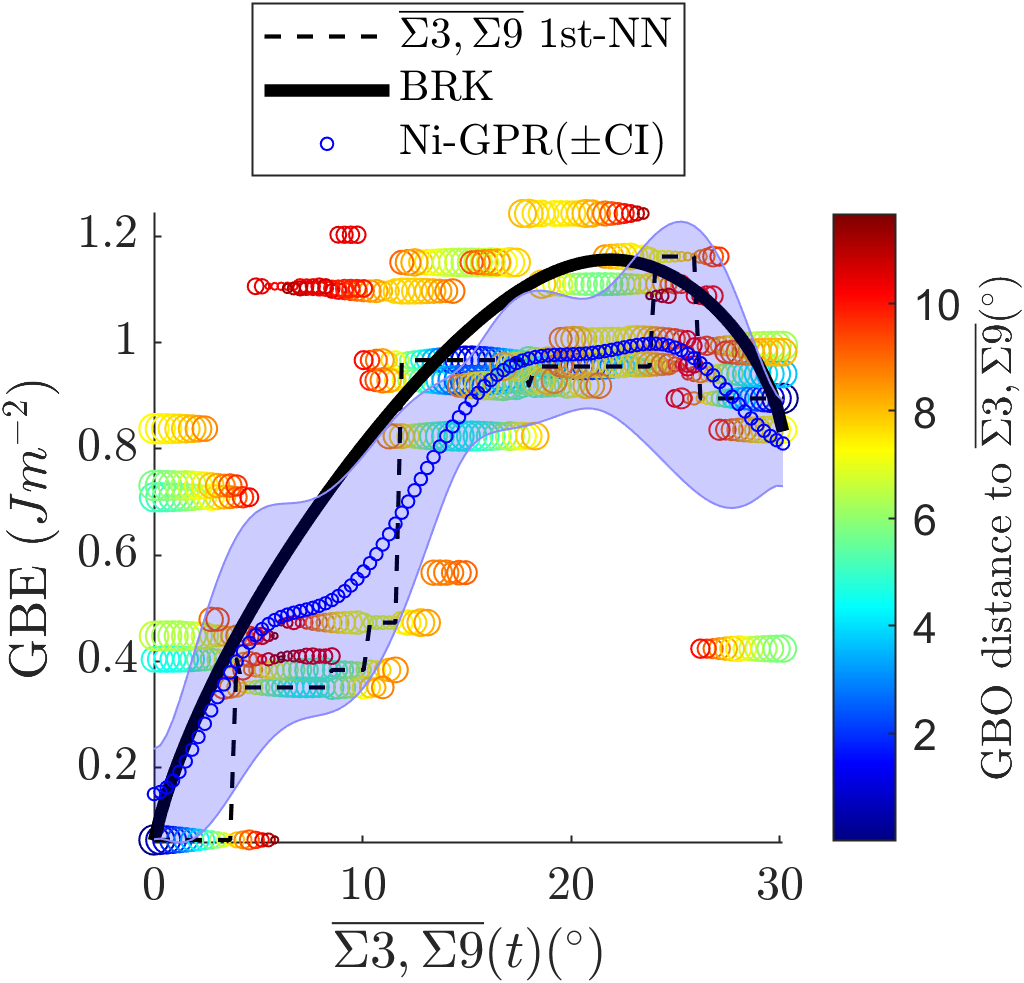
\includegraphics[width=\textwidth]{figures/tunnel-3-9-olmsted.png}
% 			\caption{}
% 			\label{fig:tunnel-3-9-olmsted}
% 		\end{subfigure}
% 		\hfill
% 		\begin{subfigure}[b]{0.48\textwidth}
% 			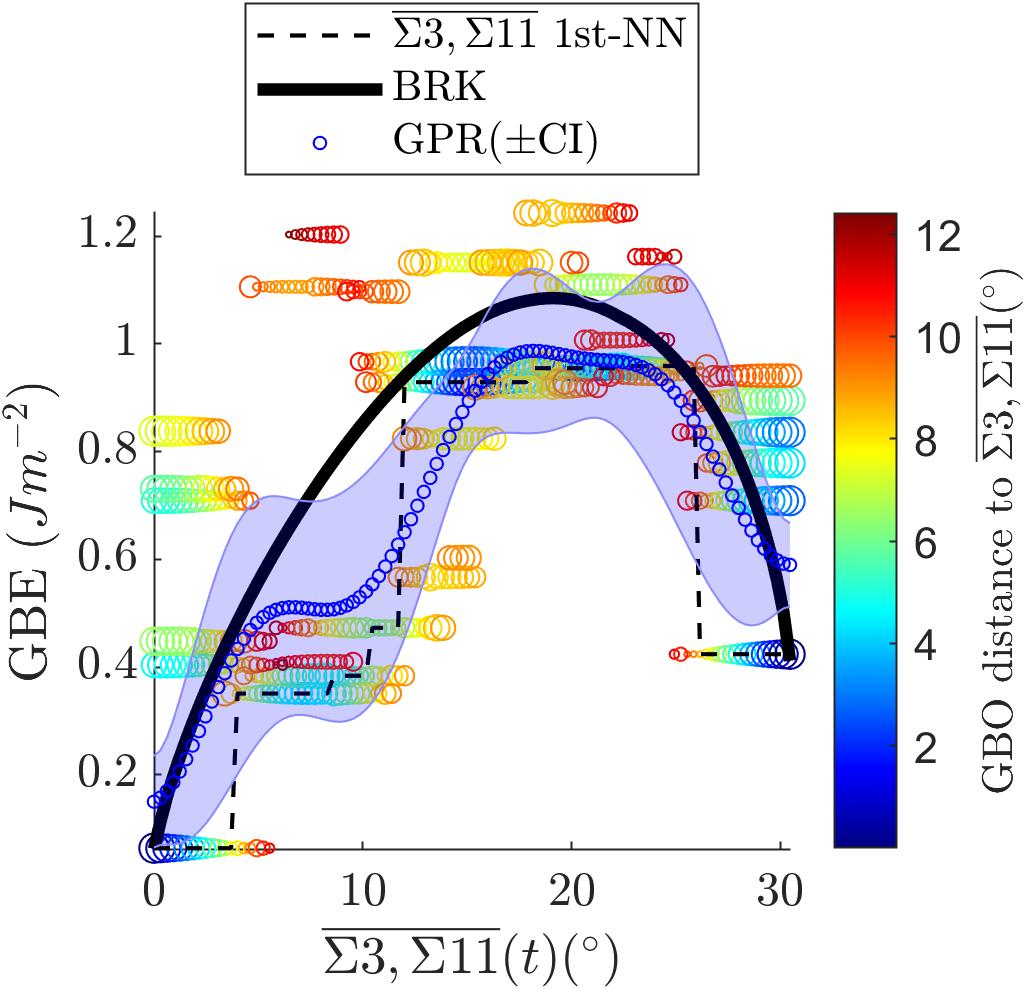
\includegraphics[width=\textwidth]{figures/tunnel-3-11-olmsted.png}
% 			\caption{}
% 			\label{fig:tunnel-3-11-olmsted}
% 		\end{subfigure}
% 		\caption{\Glspl{gbe} along direct paths in a \gls{vfz} between the $\Sigma3$ \gls{ct} boundary and minimum \gls{gbe} (\subref*{fig:tunnel-3-5-olmsted}) $\Sigma5$, (\subref*{fig:tunnel-3-7-olmsted}) $\Sigma7$, (\subref*{fig:tunnel-3-9-olmsted}) $\Sigma9$, and (\subref*{fig:tunnel-3-11-olmsted}) $\Sigma11$ \glspl{gb} within the Ni \citet{olmstedSurveyComputedGrain2009} dataset. \Gls{gbe} values are plotted for the \gls{brk} and \gls{gpr} models which both used \citet{olmstedSurveyComputedGrain2009} as \inpt{} data. }
% 		\label{fig:sigma-tunnels-olmsted}
% 	\end{figure*}
	
% 	Likewise, we perform \gls{gpr} for the Fe simulation dataset.
	
% 	\begin{figure*}[!htb]
% 		\centering
% 		\begin{subfigure}[b]{0.48\textwidth}
% 			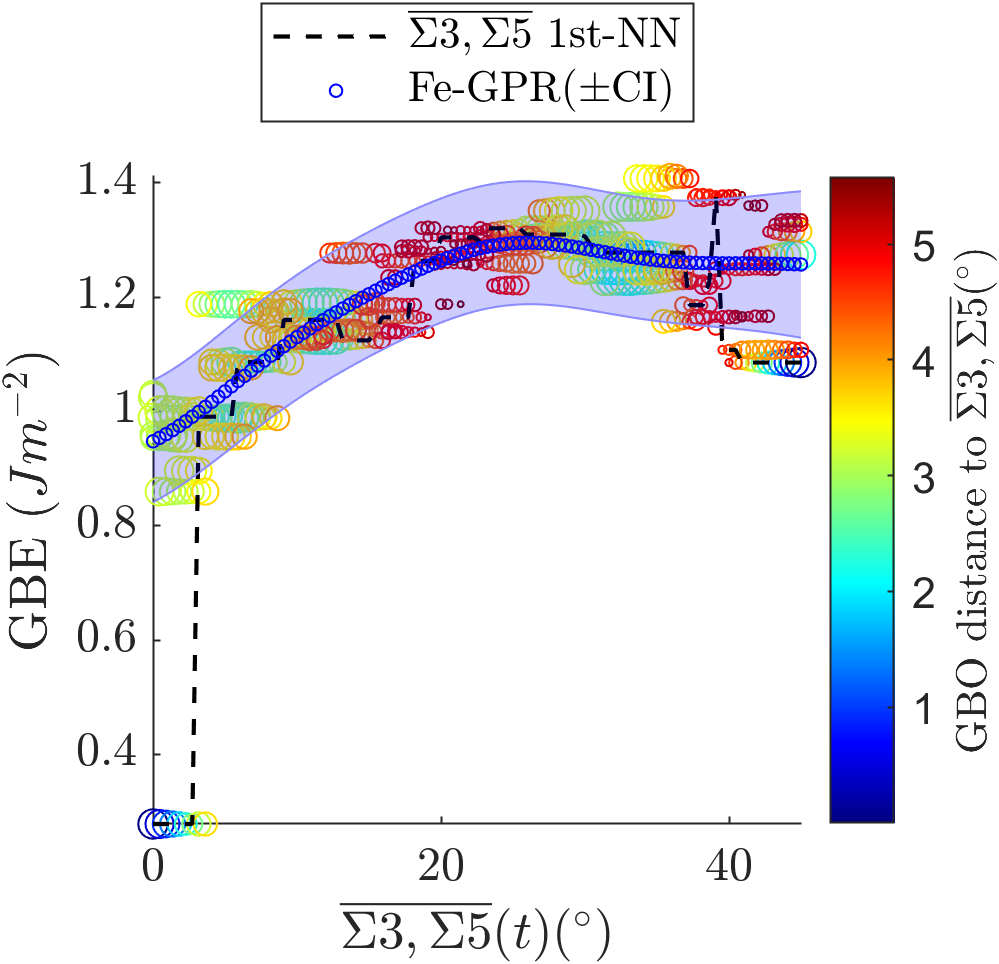
\includegraphics[width=\textwidth]{figures/tunnel-3-5-kim.png}
% 			\caption{}
% 			\label{fig:tunnel-3-5-kim}
% 		\end{subfigure}
% 		\hfill
% 		\begin{subfigure}[b]{0.48\textwidth}
% 			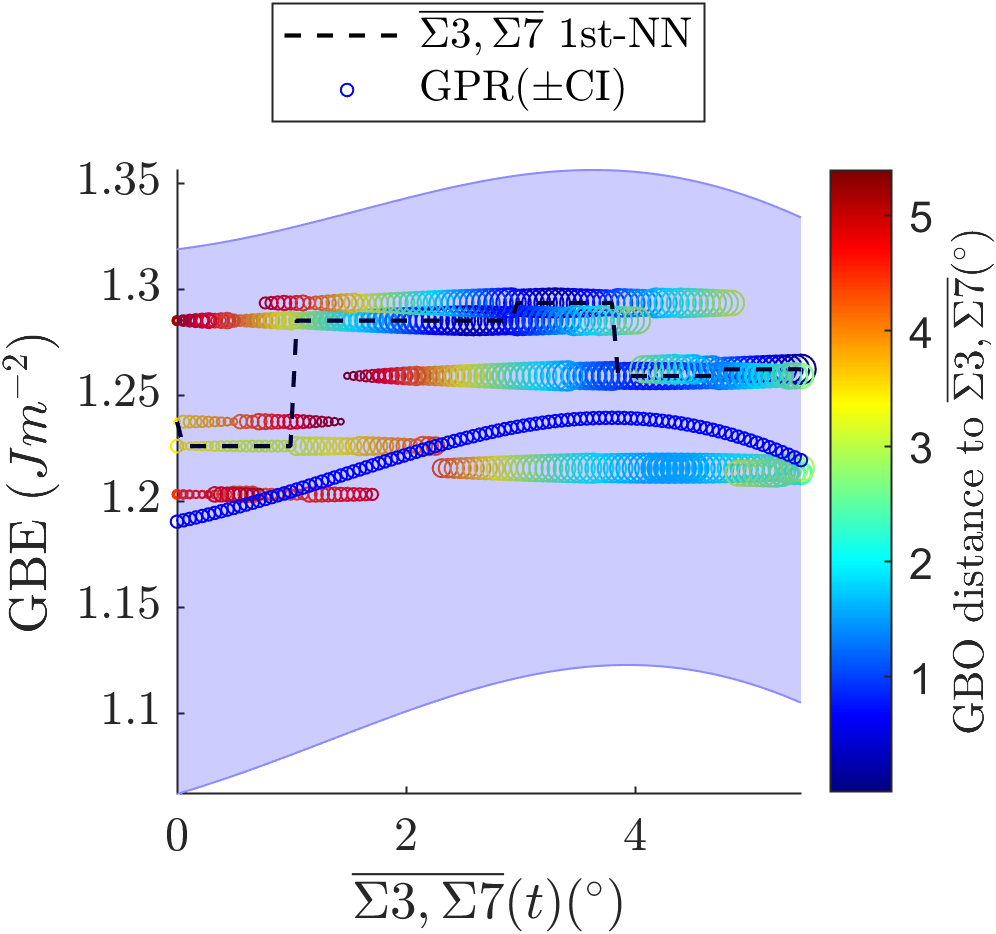
\includegraphics[width=\textwidth]{figures/tunnel-3-7-kim.png}
% 			\caption{}
% 			\label{fig:tunnel-3-7-kim}
% 		\end{subfigure}
		
% 		\begin{subfigure}[b]{0.48\textwidth}
% 			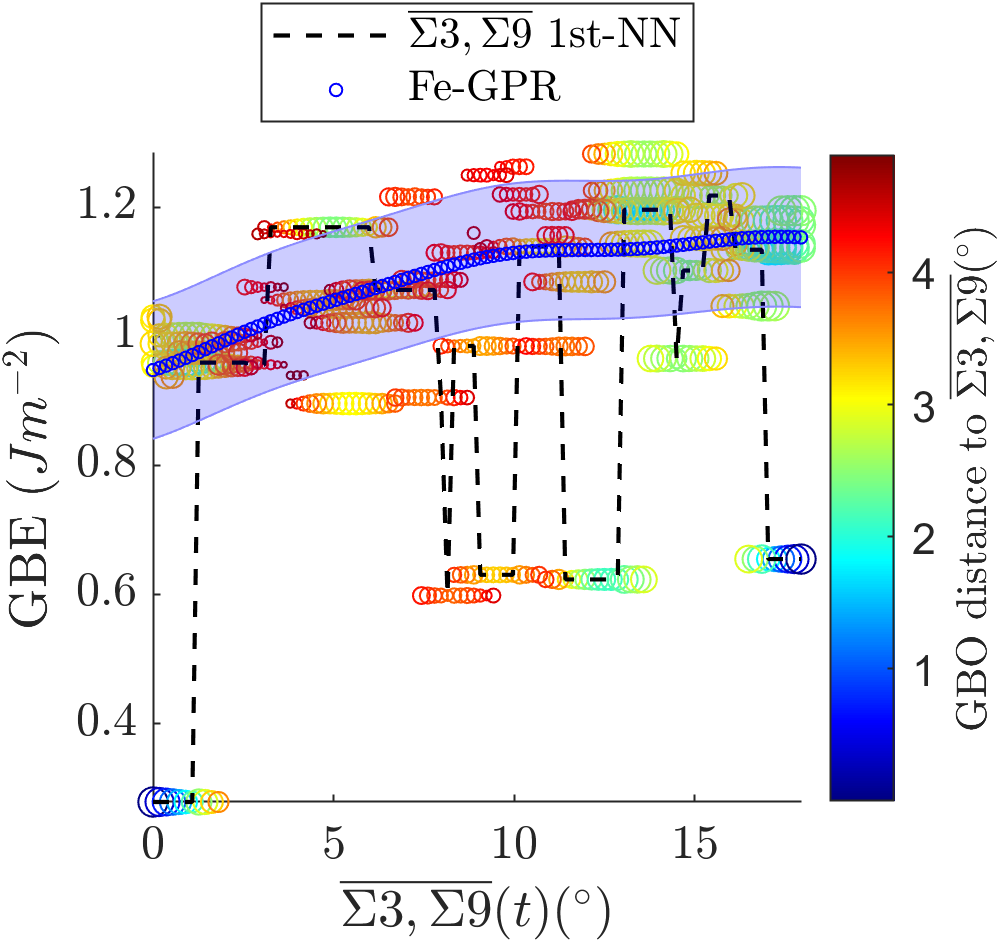
\includegraphics[width=\textwidth]{figures/tunnel-3-9-kim.png}
% 			\caption{}
% 			\label{fig:tunnel-3-9-kim}
% 		\end{subfigure}
% 		\hfill
% 		\begin{subfigure}[b]{0.48\textwidth}
% 			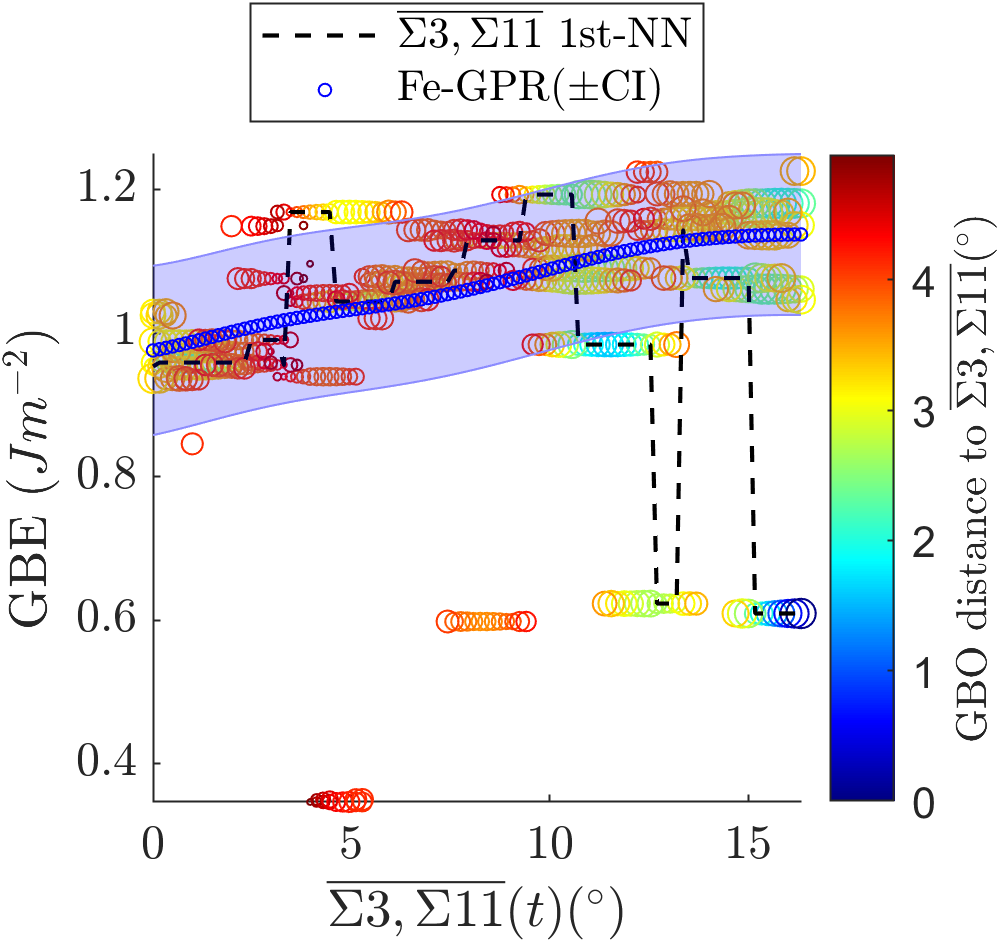
\includegraphics[width=\textwidth]{figures/tunnel-3-11-kim.png}
% 			\caption{}
% 			\label{fig:tunnel-3-11-kim}
% 		\end{subfigure}
% 		\caption{\Glspl{gbe} along direct paths in a \gls{vfz} between the $\Sigma3$ \gls{ct} boundary and minimum \gls{gbe} (\subref*{fig:tunnel-3-5-kim}) $\Sigma5$, (\subref*{fig:tunnel-3-7-kim}) $\Sigma7$, (\subref*{fig:tunnel-3-9-kim}) $\Sigma9$, and (\subref*{fig:tunnel-3-11-kim}) $\Sigma11$ \glspl{gb} for the Ni \citet{olmstedSurveyComputedGrain2009} dataset, but sampled from a \gls{gpr} model trained on \num{46883} Fe \citet{kimPhasefieldModeling3D2014} simulation datapoints. }
% 		\label{fig:sigma-tunnels-kim}
% 	\end{figure*}

\section{Gridded Sampling for Numerical Differentation} \label{sec:supp:grid}
Related to \cref{sec:results:dimensions}, an isotropically sized \gls{fz} may be easier to uniformly discretize than a high aspect-ratio space (i.e. a fixed discretization length can be used across all dimensions). What this doesn't describe, however, is curvature. In order to create a gridded array, which is important for numerical differentiation, a hypercube with each primary axis oriented with Euclidean dimensions is to be preferred. As curvature or misalignment is introduced as may be expected with a \gls{vfz} point cloud, \glspl{gb} outside of the \gls{vfz} will necessarily be sampled; this phenomena will be exaggerated in high dimensions\footnote{For perspective, a discretization into 9 segments (10 points) along each dimension will have a spacing of $\sim$\SI{7}{\degree} and require \num{1e5} grid points. In order to achieve a more reasonable grid spacing of $\sim$\SI{2}{\degree}, a minimum of $\sim$\num{24} discretizations (25 points) along each dimension is necessary and will produce $\sim$\num{1e7} grid points. }. Fortunately, most of the information is contained in the first five dimensions after \gls{svd} transformation (\cref{sec:results:dimensions}). Thus, the latter three dimensions can likely be ignored without substantially affecting e.g. an interpolation or numerical differentiation scheme.

\section{\glsxtrshort{gb}s Used for Path Visualization} \label{sec:supp:sigma-key}

See \cref{tab:sigma-key-olmsted} and \cref{tab:sigma-key-kim} for the \citet{olmstedSurveyComputedGrain2009} and \citet{kimPhasefieldModeling3D2014} datasets, respectively.

\begin{table}[!htb]
    \centering
    \caption{Minimum $\Sigma$ (Sigma) \glspl{gb} and corresponding IDs used for path visualization within the original \citet{olmstedSurveyComputedGrain2009} dataset. }
    \label{tab:sigma-key-olmsted}
    \csvautobooktabular{tables/sigma-key-olmsted.csv}
\end{table}

\begin{table}[!htb]
    \centering
    \caption{Minimum $\Sigma$ (Sigma) \glspl{gb} and corresponding IDs used for path visualization within the original \citet{kimPhasefieldModeling3D2014} dataset. }
    \label{tab:sigma-key-kim}
    \csvautobooktabular{tables/sigma-key-kim.csv}
\end{table}

\clearpage
\bibliographystyle{elsarticle-num-names}
\bibliography{5dof-gb-energy.bib}

\end{document}